\chapter{Methodology} \label{chp:methods}

\section{Statistical Modeling of Intensity SAR
data}\label{statistical-modeling-of-intensity-sar-data}

The primary models for intensity SAR data include the Gamma and
\(\mathcal{G}_I^0\) distributions~\citep{Frery1997}. The first is
suitable for fully developed speckle and is a limiting case of the
second model. This is interesting due to its versatility in accurately
representing regions with different roughness
properties~\citep{Cassetti2022}. We denote
\(Z \sim \Gamma_{\text{SAR}}(L, \mu)\) and
\(Z \sim \mathcal{G}_I^0(\alpha, \gamma, L)\) to indicate that \(Z\)
follows the distributions characterized by the respective probability
density functions (pdfs): \begin{align}
    f_Z(z;L, \mu\mid \Gamma_{\text{SAR}})&=\frac{L^L}{\Gamma(L)\mu^L}z^{L-1}\exp\left\{-Lz/\mu\right\} \mathbbm 1_{\mathbbm R_+}(z)\label{E:gamma1}\\
    \intertext{ and }
    f_Z(z; \alpha, \gamma, L \mid \mathcal{G}_I^0)&=\frac{L^L\Gamma(L-\alpha)}{\gamma^{\alpha}\Gamma(-\alpha)\Gamma(L)}\cdot\frac{z^{L-1}}{(\gamma+Lz)^{L-\alpha}} \mathbbm 1_{\mathbbm R_+}(z),\label{E:gi01}
\end{align} where \(\mu > 0\) is the mean, \(\gamma > 0\) is the scale,
\(\alpha < 0\) measures the roughness, \(L \geq 1\) is the number of
looks, \(\Gamma(\cdot)\) is the gamma function, and
\(\mathbbm 1_{A}(z)\) is the indicator function of the set \(A\).

The \(r\)th order moments of the \(\mathcal{G}_I^0\) model are
\begin{equation}
E\big(Z^r\mid \mathcal{G}_I^0\big)  = \left(\frac{\gamma}{L}\right)^r\frac{\Gamma(-\alpha-r)}{\Gamma(-\alpha)}\cdot\frac{\Gamma(L+r)}{\Gamma(L)}, 
    \label{E:rmom}
\end{equation} provided \(\alpha <-r\), and infinite otherwise.
Therefore, assuming \(\alpha<-1\), its expected value is
\begin{equation}
    \mu=\left(\frac{\gamma}{L}\right)\frac{\Gamma(-\alpha-1)}{\Gamma(-\alpha)}\cdot\frac{\Gamma(L+1)}{\gamma(L)}=-\frac{\gamma}{\alpha+1}.
\end{equation}

Although the \(\mathcal{G}_I^0\) distribution is defined by the
parameters \(\alpha\) and \(\gamma\), in the SAR
literature~\citep{Nascimento2010} the texture \(\alpha\) and the mean
\(\mu\) are usually used. 
Reparametrizing~\eqref{E:gi01} with \(\mu\),
and denoting this model as \(G_I^0\) we obtain: 
\begin{equation}
        f_Z\big(z; \mu, \alpha, L\mid G_I^0\big) = \frac{L^L\Gamma(L-\alpha)}{\big[-\mu(\alpha+1)\big]^{\alpha}\Gamma(-\alpha)\Gamma(L)} \frac{z^{L-1}}{\big[-\mu(\alpha+1)+Lz\big]^{L-\alpha}}.\label{E:gi02}
\end{equation}


\section{The Shannon Entropy}\label{the-shannon-entropy}

The parametric representation of Shannon entropy for a system described
by a continuous random variable is: \begin{equation}
  \label{E:entropy2}
  H(Z)=-\int_{-\infty }^\infty \ f(z)\ln f(z)\, \mathrm{d}z,
\end{equation} here, \(f(\cdot)\) is the pdf that characterizes the
distribution of the real-valued random variable \(Z\).

Using~\eqref{E:entropy2}, we obtain the Shannon entropy of \(\Gamma_{\text{SAR}}\) in~\eqref{E:gamma1} and \(G_I^0\) in~\eqref{E:gi02}:
\begin{equation}
\label{E:E-gamma}
H_{\Gamma_{\text{SAR}}}(L, \mu) =   L -\ln L+\ln\Gamma(L)+(1-L)\psi^{(0)}(L) + \ln \mu, 
\end{equation}
 %\begin{multline}
%\label{E:E-GIO}
%H_{\mathcal{G}_I^0}(\mu, \alpha, L) =\underbrace{L -\ln L+\ln\Gamma(L)+(1-L)\psi^{(0)}(L) +\ln \mu}_{H_{\Gamma_{\text{SAR}}}} \\
%- \underbrace{\ln\Gamma(L-\alpha)+ (L-\alpha) \psi^{(0)}(L-\alpha)-(1-\alpha)\psi^{(0)}(-\alpha)+\ln (-1-\alpha)+\ln\Gamma(-\alpha)-L}_{\phi(\alpha)},
%\end{multline} 
\begin{multline}
\label{E:E-GIO}
H_{G_I^0}(\mu, \alpha, L) =\underbrace{L -\ln L+\ln\Gamma(L)+(1-L)\psi^{(0)}(L) +\ln \mu}_{H_{\Gamma_{\text{SAR}}}} -\ln\Gamma(L-\alpha)\\
+ (L-\alpha) \psi^{(0)}(L-\alpha)-(1-\alpha)\psi^{(0)}(-\alpha)+\ln (-1-\alpha)+\ln\Gamma(-\alpha)-L,
\end{multline}
where \(\psi^{(0)}(\cdot)\) is the digamma function. 
 
Figure~\ref{fig:all_H} \ref{fig:H1} shows the theoretical entropy $H_{\Gamma_{\text{SAR}}}(L, \mu)$ as a function of $\mu$ for different values of $L$, while Figure~\ref{fig:all_H} \ref{fig:H2} shows the theoretical entropy $H_{G_I^0}(\mu, \alpha, L)$ as a function of both $\mu$ and $\alpha$, likewise considering varying $L$. 
\begin{figure}[htb]
  \centering
  \begin{subfigure}[b]{0.35\textwidth}
    \centering
    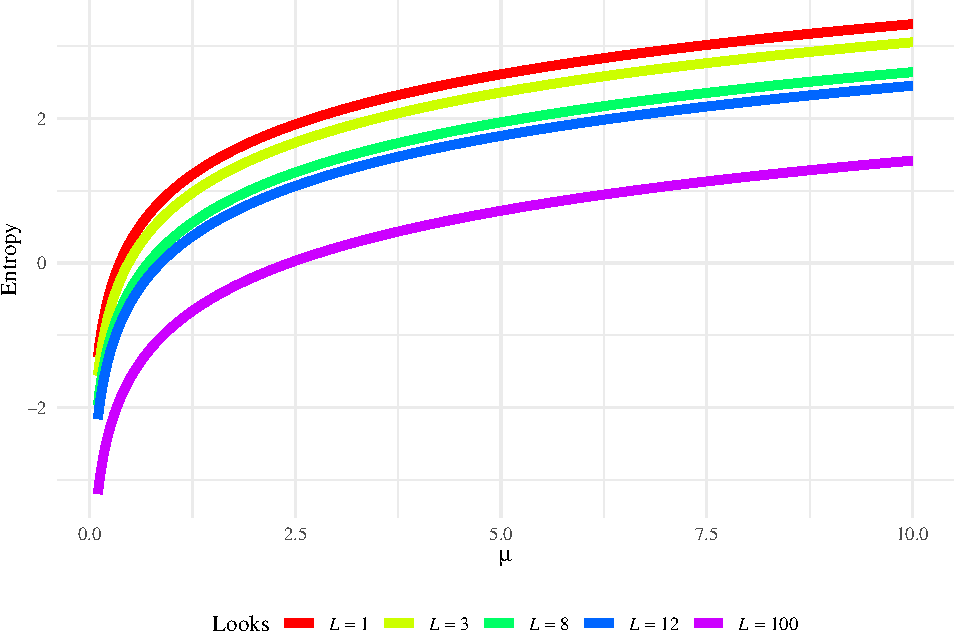
\includegraphics[width=1.5\textwidth]{../../Figures/PDF/PlotGammaSAR-1}
    \caption{The Shannon Entropy of $\Gamma_{\text{SAR}}$.}
    \label{fig:H1}
  \end{subfigure}
  \hfill
  \begin{subfigure}[b]{0.6\textwidth}
    \centering
    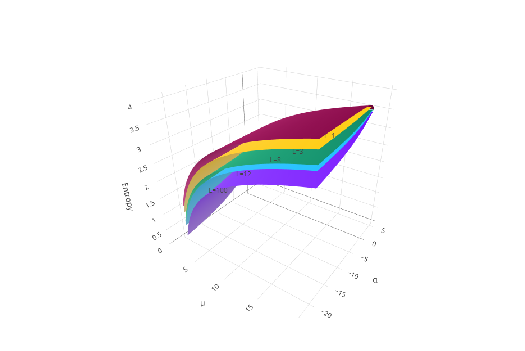
\includegraphics[width=12cm, height=7cm]{../../Figures/PDF/3d_lab}
    \caption{The Shannon Entropy of $G_I^0$.}
    \label{fig:H2}
  \end{subfigure}
  \caption{Theoretical entropies for $\Gamma_{\text{SAR}}$ and $G_I^0$ distributions.}
  \label{fig:all_H}
\end{figure}
We see that the entropy of a random variable following the $\Gamma_{\text{SAR}}$ model depends on the logarithm of the mean $\mu$.  
From the 3D plot, we observe how variations in $\mu$, $\alpha$, and $L$ collectively affect the entropy of the $G_I^0$ distribution, allowing  the identification of regions of high or low entropy.

Additionally, the expression~\eqref{E:E-GIO} can be written as: $H_{G_I^0}(\mu, \alpha, L)=H_{\Gamma_{\text{SAR}}}+\phi(\alpha, L)$. Thus, for $L\geq1$ known, and as \(\alpha\to-\infty\) we have that $H_{G_I^0}\approx H_{\Gamma_{\text{SAR}}}$. 
Figure~\ref{fig:Plot_GI0_to_gamma1}, shows the behavior of the entropy
of \(G_I^0\) as a function of $\mu$ when \(\alpha \in \left\{-\infty, -20, -8, -3\right\}\) and $L=8$,
where the approximation to the entropy of \(\Gamma_{\text{SAR}}\) can be
observed when \(\alpha\) assumes large negative values. In an
interpretative sense, we can conclude that the more heterogeneous (high
values of \(\alpha\)) the SAR region is, the higher the value of entropy
(or degree of disorder). It is worth noting that this conclusion
confirms what is written in the SAR literature.


\begin{figure}[htb]

{\centering 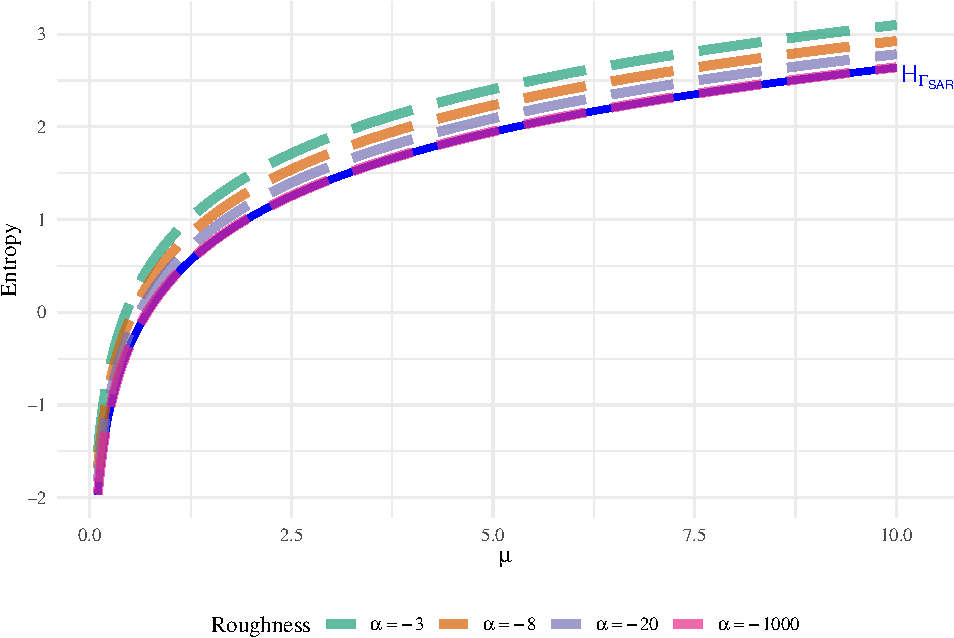
\includegraphics[width=0.7\linewidth]{../../Figures/PDF/Plot_GI0_to_gamma1-1} 

}

\caption{$H_{ G_I^0}$ converges to the $H_{\Gamma_{\text{SAR}}}$ when $\alpha\to-\infty$, with $L=8$.}\label{fig:Plot_GI0_to_gamma1}
\end{figure}

\subsection{Estimation of the Shannon
Entropy}\label{estimation-of-the-shannon-entropy}

The problem of the non-parametric estimation of \(H(Z)\) has been
studied by many authors,
including~\citep{vasicek1976test,correa1995new,Wieczorkowski1999,Yee2015,AlOmari2019}.
Their proposals use estimators based on differences between order
statistics: spacings.

\citet{vasicek1976test} introduced one of the first
non-parametric estimators based on spacings. Under the assumption that
\(\bm{Z}=(Z_1, Z_2,\ldots,Z_n)\) is a random sample from the
distribution \(F(z)\), the estimator is defined as: \begin{equation}
\label{E:Vas}
    \widehat{H}_{\text{V}}(\bm{Z})=\frac{1}{n}\sum_{i=1}^{n}\ln\left[\frac{n}{2m}\left(Z_{(i+m)}-Z_{(i-m)}\right)\right],
    \end{equation} where \(m<n/2\) is a positive integer,
\(Z_{(1)}\leq Z_{(2)}\leq\dots\leq Z_{(n)}\) are the order statistics,
and \(Z_{(i+m)}-Z_{(i-m)}\) is the \(m\)-spacing, in which
\(Z_{(i)}= Z_{(1)}\) if \(i<1\), \(Z_{(i)}= Z_{(n)}\) if \(i>n\).

Several authors have explored adaptations  to Vasicek's estimator. We consider the following entropy estimators variants, as discussed by~\citep{AlOmari2016,Cassetti2022}.

\citet{Bert1992} proposed a new estimator of entropy given by:
 \begin{equation}
\label{E:VanEs}
	\widehat{H}_{\text{VE}}(\bm{Z})=\frac{1}{n-m}\sum_{i=1}^{n-m}\log\left[\frac{n+1}{m}\left(Z_{(i+m)}-Z_{(i)}\right)\right]	+\sum_{k=m}^n\frac{1}{k}+\log\frac{m}{n+1}.
\end{equation}
Under some conditions, Van Es proved asymptotic normality of this estimator.

\citet{Ebrahimi1994} adjusted the weights of Vasicek's estimator, in order to take into account the fact that the differences are truncated around the smallest and the largest data points.
 Specifically, $Z_{(i+m)}-Z_{(i-m)}$ is substituted with  $Z_{(i+m)}-Z_{(1)}$ when $i \leq m$ and $Z_{(i+m)}-Z_{(i-m)}$ is replaced by $Z_{(n)}-Z_{(i-m)}$ when $i \geq n-m+1$. Their estimator is given by:
  \begin{equation}
	\label{E:Ebrahimi}
  \widehat{H}_{\text{E}}(\bm{Z})=\frac{1}{n} \sum_{i=1}^n \log \left[\frac{n}{c_i m}\left(Z_{(i+m)}-Z_{(i-m)}\right)\right],
  \end{equation} where \[
  c_i=\begin{cases}1+(i-1) / m & \text { if } \quad 1 \leq i \leq m, \\ 2 & \text { if }\quad m+1 \leq i \leq n-m,\\ 1+(n-i) / m & \text { if }\quad n-m+1 \leq i \leq n.\end{cases}
  \]

 \citet{correa1995new} suggested another modification of Vasicek's estimator. 
In estimation the density $f$ of $F$ in the interval $\left(Z_{(i-m)}, Z_{(i+m)}\right)$ he used a local linear model based on $2 m+1$ points: $F\left(Z_{(j)}\right)=a+b Z_{(j)}+\varepsilon, j=m-i, \ldots, m+i$. This yields a following estimator:
  \begin{equation}
	\label{E:Correa}
  \widehat{H}_{\text{C}}(\bm{Z})=-\frac{1}{n} \sum_{i=1}^n \log \frac{\sum_{j=i-m}^{i+m}(j-i)\left(Z_{(j)}-\overline{Z}_{(i)}\right)}{n\sum_{j=i-m}^{i+m}\left(Z_{(j)}-\overline{Z}_{(i)}\right)^2},
  \end{equation} where
  \(\widebar{Z}_{(i)}=(2 m+1)^{-1} \sum_{j=i-m}^{i+m} Z_{(j)}\),
  \(m< \frac{n}{2}\), \(Z_{(i)}=Z_{(1)}\) for \(i<1\) and
  \(Z_{(i)}=Z_{(n)}\) for \(i>n\). Based on simulations, he showed that
  his estimator has a smaller mean square error than Vasicek's approach.
	
	 
\citet{rohtua} modify the coefficients of~\eqref{E:Ebrahimi} as: 
\begin{equation}
\label{E:NA}
\widehat{H}_{\text{NA}}(\bm{Z})=\frac{1}{n} \sum_{i=1}^n \log \left[\frac{n}{a_i m}\left(Z_{(i+m)}-Z_{(i-m)}\right)\right],
\end{equation}
where
$$
a_i=\begin{cases}
1 & \text { if } \quad 1 \leq i \leq m, \\
2 & \text { if } \quad m+1 \leq i \leq n-m, \\
1 & \text { if } \quad n-m+1 \leq i \leq n,
\end{cases}
$$
and $Z_{(i-m)}=Z_{(1)}$ for $i \leq m$ and $Z_{(i+m)}=Z_{(n)}$ for $i \geq n-m$.

\citet{IbrahimAlOmari2014} suggested the following estimator:
	\begin{equation}
\label{E:AO}
  \widehat{H}_{\text{AO}}(\bm{Z})=\frac{1}{n} \sum_{i=1}^n \log \left[\frac{n}{\omega_i m}\left(Z_{(i+m)}-Z_{(i-m)}\right)\right],
 \end{equation}
	where \[
  \omega_i= \begin{cases}3/2 & \text { if }\quad 1 \leq i \leq m, \\ 2 & \text { if }\quad m+1 \leq i \leq n-m, \\ 3/2 & \text { if } \quad n-m+1 \leq i \leq n,\end{cases}
  \] in which \(Z_{(i-m)}=Z_{(1)}\) for \(i \leq m\), and
  \(Z_{(i+m)}=Z_{(n)}\) for \(i \geq n-m\).


These estimators are asymptotically consistent, i.e., they converge in
probability to the true value when \(m,n\rightarrow\infty\) and
\(m/n\rightarrow0\). 



Our experimental setup involves an analysis of bias and mean squared error (MSE) for each estimator with a Monte Carlo
study, using \(1000\) samples from the \(\Gamma_{\text{SAR}}\) distribution of size
\(n\in\left\{9, 25, 49, 81, 121\right\}\), with
\(\mu\in\left\{1, 10, 50, 100\right\}\) and \(L=5\). 
The results are consistent with other situations. We use the
heuristic spacing \(m=\left[\sqrt{n}+0.5\right]\), as recommended in the
literature.
Figure~\ref{fig:Plot_bias_mse_gi0_new_L5}  presents the bias and MSE for each of the non-parametric entropy estimators.  The results are summarized  in Table~\ref{tab:tableL5}.
%\begin{figure}[H]
%{\centering 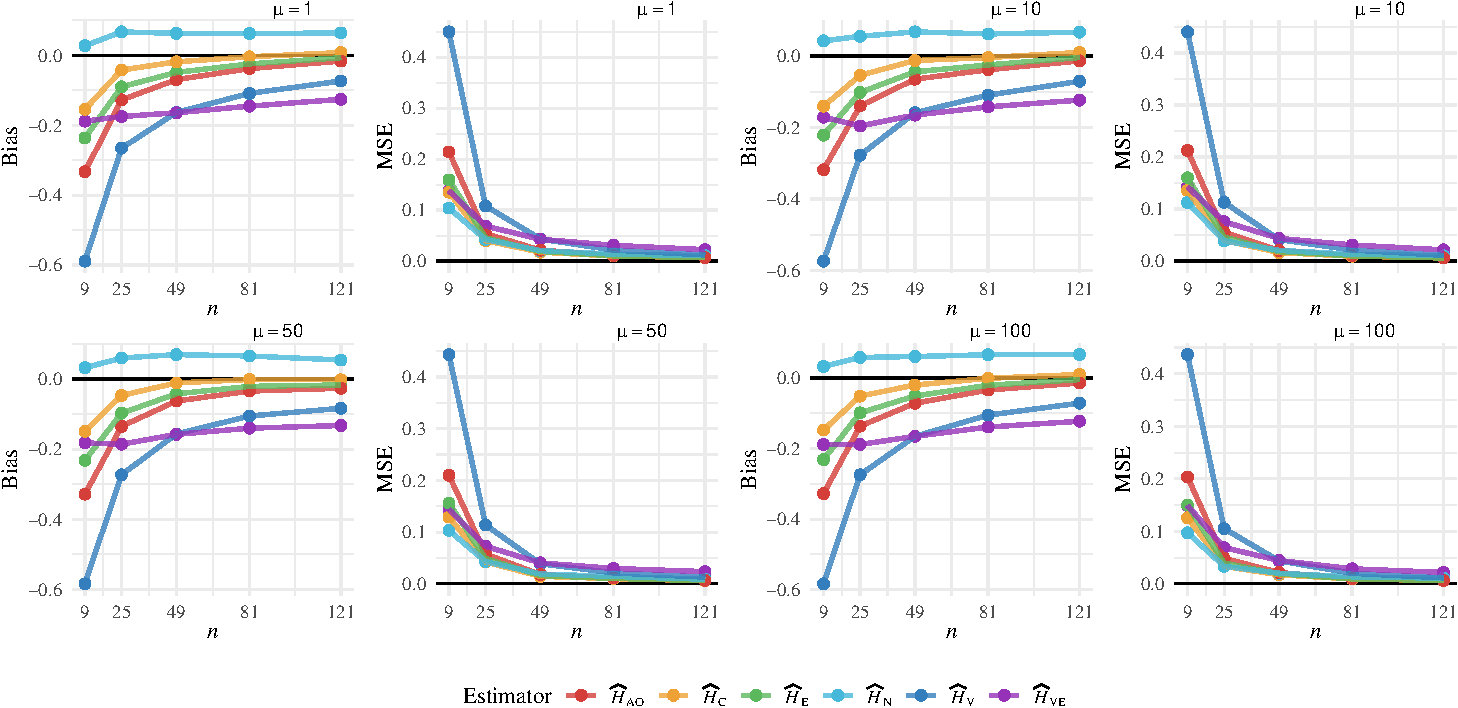
\includegraphics[width=1\linewidth]{../../Figures/PDF/Plot_bias_mse_gi0_new_L2-1} 
%
%}
%\caption{Bias and MSE of the entropy estimators for the $\Gamma_{\text{SAR}}$, with $L=2$.}\label{fig:Plot_bias_mse_gi0_new_L2}
%\end{figure}
\begin{figure}[htb]
{\centering 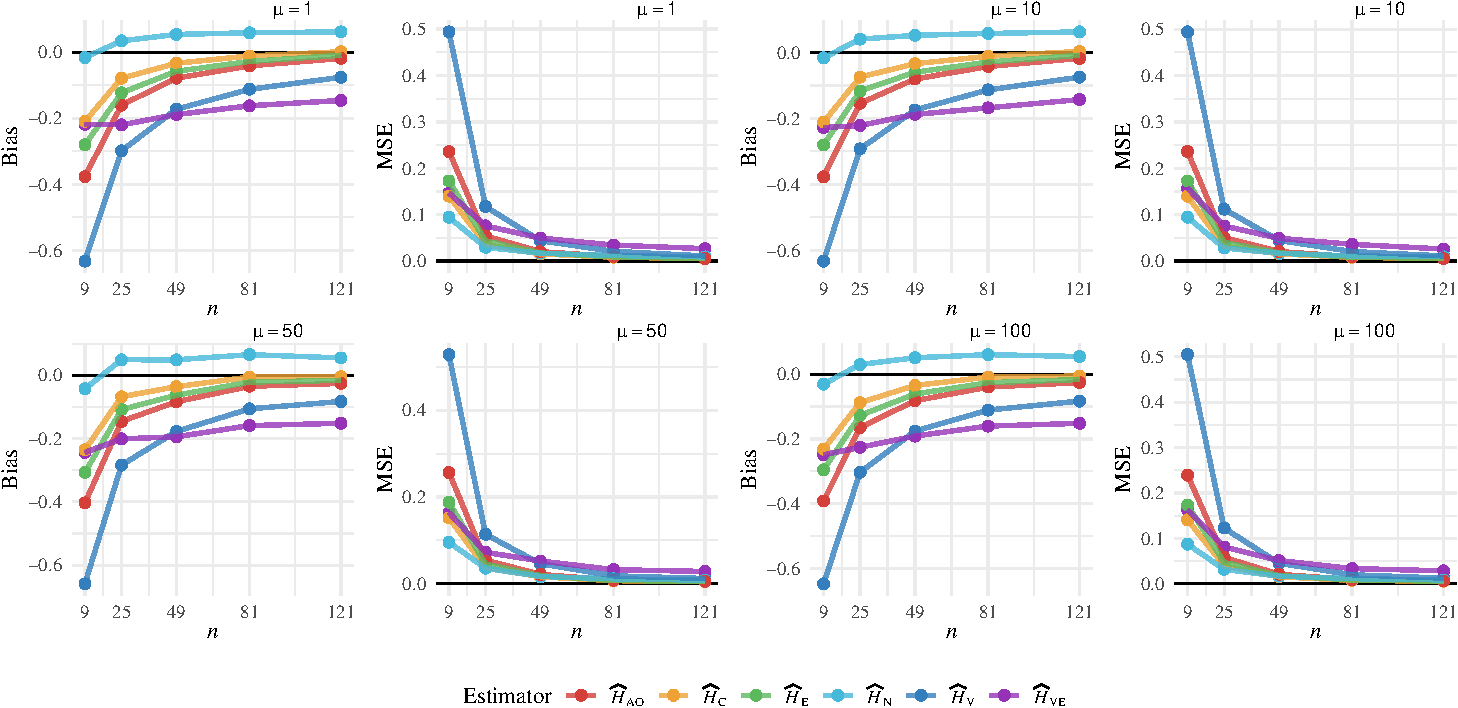
\includegraphics[width=1\linewidth]{../../Figures/PDF/Plot_bias_mse_gi0_new_L5-1} 

}
\caption{Bias and MSE of the entropy estimators for the $\Gamma_{\text{SAR}}$, with $L=5$.}\label{fig:Plot_bias_mse_gi0_new_L5}
\end{figure}



\setlength{\tabcolsep}{6pt}
\begin{table}[htb]
\centering
\caption{\label{tab:tableL5}Bias and MSE of the entropy estimators for the $\Gamma_{\text{SAR}}$, with $L=5$.}
\resizebox{\ifdim\width>\linewidth\linewidth\else\width\fi}{!}{
\begin{tabular}[t]{crllllllllllll}
\toprule
\multicolumn{1}{c}{ } & \multicolumn{1}{c}{ } & \multicolumn{6}{c}{Bias} & \multicolumn{6}{c}{MSE} \\
\cmidrule(l{3pt}r{3pt}){3-8} \cmidrule(l{3pt}r{3pt}){9-14}
\multicolumn{1}{r}{$\bm{\mu}$} & \multicolumn{1}{r}{$\bm{n}$} & \multicolumn{1}{r}{$\bm{\widehat{H}_{\text{V}}}$} & \multicolumn{1}{r}{$\bm{\widehat{H}_{\text{VE}}}$} & \multicolumn{1}{r}{$\bm{\widehat{H}_{\text{E}}}$} & \multicolumn{1}{r}{$\bm{\widehat{H}_{\text{C}}}$} & \multicolumn{1}{r}{$\bm{\widehat{H}_{\text{N}}}$} & \multicolumn{1}{r}{$\bm{\widehat{H}_{\text{AO}}}$} & \multicolumn{1}{r}{$\bm{\widehat{H}_{\text{V}}}$} & \multicolumn{1}{r}{$\bm{\widehat{H}_{\text{VE}}}$} & \multicolumn{1}{r}{$\bm{\widehat{H}_{\text{E}}}$} & \multicolumn{1}{r}{$\bm{\widehat{H}_{\text{C}}}$} & \multicolumn{1}{r}{$\bm{\widehat{H}_{\text{N}}}$} & \multicolumn{1}{r}{$\bm{\widehat{H}_{\text{AO}}}$}\\
\midrule
 & $9$ & $-0.632$ & $-0.218$ & $-0.280$ & $-0.210$ & $-0.016$ & $-0.377$ & $\phantom{-}0.494$ & $\phantom{-}0.147$ & $\phantom{-}0.173$ & $\phantom{-}0.140$ & $\phantom{-}0.094$ & $\phantom{-}0.236$\\

 & $25$ & $-0.298$ & $-0.220$ & $-0.123$ & $-0.079$ & $\phantom{-}0.034$ & $-0.160$ & $\phantom{-}0.117$ & $\phantom{-}0.076$ & $\phantom{-}0.044$ & $\phantom{-}0.036$ & $\phantom{-}0.030$ & $\phantom{-}0.054$\\

 & $49$ & $-0.173$ & $-0.189$ & $-0.058$ & $-0.033$ & $\phantom{-}0.054$ & $-0.079$ & $\phantom{-}0.044$ & $\phantom{-}0.050$ & $\phantom{-}0.017$ & $\phantom{-}0.015$ & $\phantom{-}0.017$ & $\phantom{-}0.020$\\

 & $81$ & $-0.112$ & $-0.162$ & $-0.028$ & $-0.011$ & $\phantom{-}0.059$ & $-0.041$ & $\phantom{-}0.021$ & $\phantom{-}0.035$ & $\phantom{-}0.009$ & $\phantom{-}0.008$ & $\phantom{-}0.012$ & $\phantom{-}0.010$\\

\multirow{-5}{*}[2\dimexpr\aboverulesep+\belowrulesep+\cmidrulewidth]{\centering\arraybackslash 1} & $121$ & $-0.076$ & $-0.146$ & $-0.009$ & $\phantom{-}0.001$ & $\phantom{-}0.061$ & $-0.019$ & $\phantom{-}0.011$ & $\phantom{-}0.027$ & $\phantom{-}0.005$ & $\phantom{-}0.005$ & $\phantom{-}0.009$ & $\phantom{-}0.006$\\
\cmidrule{1-14}
 & $9$ & $-0.633$ & $-0.228$ & $-0.280$ & $-0.211$ & $-0.016$ & $-0.377$ & $\phantom{-}0.494$ & $\phantom{-}0.157$ & $\phantom{-}0.173$ & $\phantom{-}0.140$ & $\phantom{-}0.094$ & $\phantom{-}0.236$\\

 & $25$ & $-0.292$ & $-0.221$ & $-0.117$ & $-0.075$ & $\phantom{-}0.041$ & $-0.154$ & $\phantom{-}0.112$ & $\phantom{-}0.076$ & $\phantom{-}0.040$ & $\phantom{-}0.032$ & $\phantom{-}0.028$ & $\phantom{-}0.050$\\

 & $49$ & $-0.174$ & $-0.188$ & $-0.060$ & $-0.034$ & $\phantom{-}0.052$ & $-0.080$ & $\phantom{-}0.045$ & $\phantom{-}0.049$ & $\phantom{-}0.018$ & $\phantom{-}0.016$ & $\phantom{-}0.017$ & $\phantom{-}0.021$\\

 & $81$ & $-0.113$ & $-0.168$ & $-0.029$ & $-0.011$ & $\phantom{-}0.058$ & $-0.042$ & $\phantom{-}0.021$ & $\phantom{-}0.036$ & $\phantom{-}0.009$ & $\phantom{-}0.008$ & $\phantom{-}0.011$ & $\phantom{-}0.009$\\

\multirow{-5}{*}[2\dimexpr\aboverulesep+\belowrulesep+\cmidrulewidth]{\centering\arraybackslash 10} & $121$ & $-0.075$ & $-0.143$ & $-0.008$ & $\phantom{-}0.003$ & $\phantom{-}0.063$ & $-0.018$ & $\phantom{-}0.011$ & $\phantom{-}0.026$ & $\phantom{-}0.006$ & $\phantom{-}0.005$ & $\phantom{-}0.009$ & $\phantom{-}0.006$\\
\cmidrule{1-14}
 & $9$ & $-0.659$ & $-0.244$ & $-0.307$ & $-0.236$ & $-0.043$ & $-0.403$ & $\phantom{-}0.528$ & $\phantom{-}0.164$ & $\phantom{-}0.188$ & $\phantom{-}0.152$ & $\phantom{-}0.096$ & $\phantom{-}0.256$\\

 & $25$ & $-0.284$ & $-0.201$ & $-0.108$ & $-0.068$ & $\phantom{-}0.049$ & $-0.146$ & $\phantom{-}0.114$ & $\phantom{-}0.073$ & $\phantom{-}0.045$ & $\phantom{-}0.038$ & $\phantom{-}0.036$ & $\phantom{-}0.055$\\

 & $49$ & $-0.178$ & $-0.194$ & $-0.063$ & $-0.036$ & $\phantom{-}0.049$ & $-0.084$ & $\phantom{-}0.046$ & $\phantom{-}0.053$ & $\phantom{-}0.019$ & $\phantom{-}0.016$ & $\phantom{-}0.017$ & $\phantom{-}0.022$\\

 & $81$ & $-0.106$ & $-0.159$ & $-0.022$ & $-0.006$ & $\phantom{-}0.065$ & $-0.035$ & $\phantom{-}0.018$ & $\phantom{-}0.033$ & $\phantom{-}0.008$ & $\phantom{-}0.007$ & $\phantom{-}0.011$ & $\phantom{-}0.008$\\

\multirow{-5}{*}[2\dimexpr\aboverulesep+\belowrulesep+\cmidrulewidth]{\centering\arraybackslash 50} & $121$ & $-0.083$ & $-0.152$ & $-0.016$ & $-0.004$ & $\phantom{-}0.054$ & $-0.026$ & $\phantom{-}0.012$ & $\phantom{-}0.029$ & $\phantom{-}0.006$ & $\phantom{-}0.005$ & $\phantom{-}0.008$ & $\phantom{-}0.006$\\
\cmidrule{1-14}
 & $9$ & $-0.647$ & $-0.249$ & $-0.295$ & $-0.232$ & $-0.031$ & $-0.391$ & $\phantom{-}0.505$ & $\phantom{-}0.163$ & $\phantom{-}0.173$ & $\phantom{-}0.141$ & $\phantom{-}0.087$ & $\phantom{-}0.239$\\

 & $25$ & $-0.303$ & $-0.226$ & $-0.127$ & $-0.088$ & $\phantom{-}0.030$ & $-0.165$ & $\phantom{-}0.123$ & $\phantom{-}0.081$ & $\phantom{-}0.047$ & $\phantom{-}0.039$ & $\phantom{-}0.032$ & $\phantom{-}0.058$\\

 & $49$ & $-0.176$ & $-0.191$ & $-0.061$ & $-0.035$ & $\phantom{-}0.050$ & $-0.082$ & $\phantom{-}0.045$ & $\phantom{-}0.051$ & $\phantom{-}0.018$ & $\phantom{-}0.016$ & $\phantom{-}0.017$ & $\phantom{-}0.021$\\

 & $81$ & $-0.111$ & $-0.160$ & $-0.027$ & $-0.009$ & $\phantom{-}0.060$ & $-0.040$ & $\phantom{-}0.020$ & $\phantom{-}0.034$ & $\phantom{-}0.008$ & $\phantom{-}0.008$ & $\phantom{-}0.011$ & $\phantom{-}0.009$\\

\multirow{-5}{*}[2\dimexpr\aboverulesep+\belowrulesep+\cmidrulewidth]{\centering\arraybackslash 100} & $121$ & $-0.083$ & $-0.152$ & $-0.017$ & $-0.006$ & $\phantom{-}0.054$ & $-0.026$ & $\phantom{-}0.013$ & $\phantom{-}0.029$ & $\phantom{-}0.006$ & $\phantom{-}0.006$ & $\phantom{-}0.009$ & $\phantom{-}0.006$\\
\bottomrule
\end{tabular}}
\end{table}
As shown in the simulation results, the estimators \(\widehat{H}_{\text{C}}\), \(\widehat{H}_{\text{E}}\), and \(\widehat{H}_{\text{AO}}\) show low bias and achieve convergence for samples size larger than 81. These estimators exhibit good behavior in terms of bias and MSE across various parameter combinations.

In contrast, estimator \(\widehat{H}_{\text{N}}\) displays the lowest MSE across all scenarios. However,  the bias remains unchanged and high for sample sizes larger than 25, indicating that the convergence
is not very fast. Additionally, we observe that both \(\widehat{H}_{\text{V}}\) and \(\widehat{H}_{\text{VE}}\) estimators exhibit larger bias and slower convergence compared to their counterparts.  Notably, the \(\widehat{H}_{\text{V}}\) estimator shows the highest MSE.

%We will use improved bootstrap-improved versions because we need them to perform well with small samples.

\subsection{Enhanced estimators with Bootstrap}\label{enhanced-estimators-with-bootstrap}

We extend our exploration of non-parametric entropy estimators by incorporating  bootstrap methodologies, because we need them to perform well with small samples. 
The integration of bootstrap techniques aims to refine the accuracy of non-parametric entropy estimators.

Bootstrap is essentially a resampling algorithm introduced by \citep{Efron1979}. 
It offers a simulation-based approach for estimating various statistics of interest for a random variable.
It can be used in both parametric and nonparametric settings. 
The main idea  consists of creating new datasets from an existing one by resampling with repetition~\citep{Michelucci2021}.

Let us assume that the non-parametric entropy estimator
\(\widehat{H}=\widehat{\theta}(\bm{Z})\) is inherently biased, where \(\bm{Z}=(Z_1, Z_2,\ldots,Z_n)\) is a random sample from a
distribution \(\mathcal{D}\), i.e,:\begin{equation}
\label{Eq:bias1}
\operatorname{Bias}\big(\widehat{\theta}(\bm{Z})\big) = \mathbb{E}\big[\widehat{\theta}(\bm{Z})\big] - \theta \neq 0.
\end{equation} 

Our objective is to devise a unbiased estimator. To achieve this, we introduce an "ideal estimator" \(\widecheck{\theta}(\bm{Z})\) using the bias information from~\eqref{Eq:bias1}:
\begin{align}
\label{Eq:bias2}
\widecheck{\theta}(\bm{Z}) &= \widehat{\theta}(\bm{Z}) - \bias\left(\widehat{\theta}(\bm{Z})\right),\nonumber\\
&=\widehat{\theta}(\bm{Z})-\left[\mathbb{E}\big[\widehat{\theta}(\bm{Z})\big] - \theta\right],\nonumber\\
&=\widehat{\theta}(\bm{Z})+\theta-\mathbb{E}\big[\widehat{\theta}(\bm{Z})\big].
\end{align}
However, \(\widecheck{\theta}(\bm{Z})\) is not yet an estimator, because it depend on the true parameter, but \(\theta\) can be calculated using a non-parametric approach, and the average of individual estimators can be obtained using the bootstrap technique. This leads to the formulation of a new unbiased estimator, denoted as \(\widetilde{H}\), from ~\eqref{Eq:bias2} we have:
\begin{align}
\label{Eq:bias3}
\widetilde{H}%&= \widehat{\theta}(\bm{Z})+\widehat{\theta}(\bm{Z})- \frac{1}{B}\sum_{b=1}^B \widehat{\theta}_b(\bm{Z}^{(b)}),\nonumber\\
= 2\widehat{\theta}(\bm{Z}) - \frac{1}{B}\sum_{b=1}^B \widehat{\theta}_b(\bm{Z}^{(b)}),
\end{align} where \(B\) the number of bootstrap replications. For each iteration \(b\) (from \(1\) to \(B\)), a sample \(\bm{Z}^{(b)}\) is generated, and the corresponding bootstrap estimator \(\widehat{\theta}_b(\bm{Z}^{(b)})\) is calculated. 
This methodology significantly reduces bias, resulting in more accurate and robust entropy estimations. The original estimators of Vasicek~\eqref{E:Vas}, Van Es~\eqref{E:VanEs}, Ebrahimi~\eqref{E:Ebrahimi}, Correa~\eqref{E:Correa}, Noughabi~\eqref{E:NA}, and Al-Omari~\eqref{E:AO}  are now referred to as the proposed bootstrap-improved versions:
\(\widetilde{H}_{\text{V}}\),
\(\widetilde{H}_{\text{VE}}\), 
\(\widetilde{H}_{\text{E}}\),
\(\widetilde{H}_{\text{C}}\),
\(\widetilde{H}_{\text{NA}}\), and 
\(\widetilde{H}_{\text{AO}}\),
respectively.

In order to assess the effectiveness of the bootstrap technique, we present comparisons of the bias and MSE between each original non-parametric entropy estimator and its respective bootstrap-enhanced version, with \(B=200\) bootstrap samples, as shown in Figures~\ref{fig:all_estimator}~\ref{fig:Firstfigure}--\ref{fig:subfig6}.
\begin{figure}[H]
  \centering
  \begin{subfigure}[t]{0.48\textwidth}
    \centering
    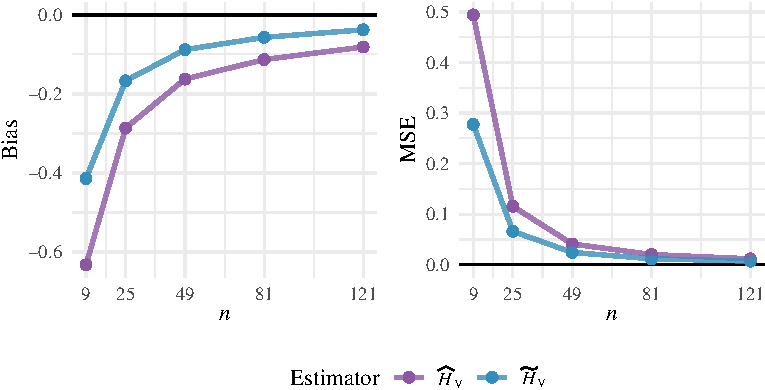
\includegraphics[width=\textwidth]{../../Figures/PDF/Plot_bias_mse_vasicek-1}
    \caption{}
    \label{fig:Firstfigure}
  \end{subfigure}
  \hfill
  \begin{subfigure}[t]{0.48\textwidth}
    \centering
    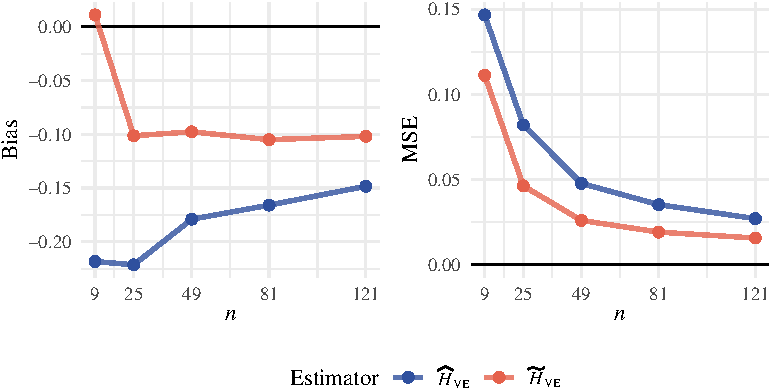
\includegraphics[width=\textwidth]{../../Figures/PDF/Plot_bias_mse_VanEs-1}
    \caption{}
    \label{fig:Secondfigure}
  \end{subfigure}
  %\hfill
  %\begin{subfigure}[b]{0.3\textwidth}
    %\centering
    %\includegraphics[width=\textwidth]{example-image-c}
    %\caption{}
    %\label{fig: Third figure}
  %\end{subfigure}
	
	\begin{subfigure}[t]{0.48\textwidth}
    \centering
    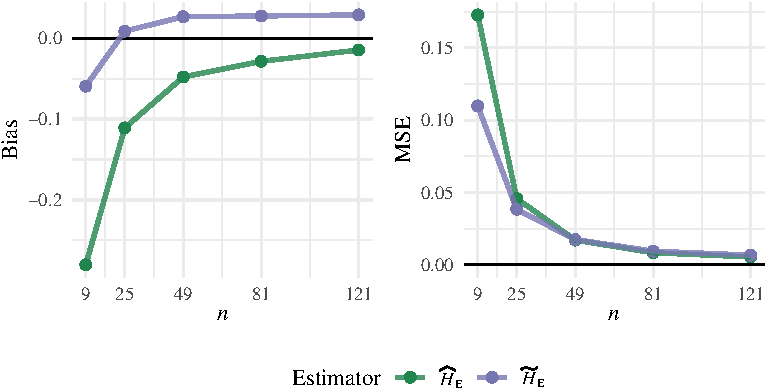
\includegraphics[width=\textwidth]{../../Figures/PDF/Plot_bias_mse_Ebrahimi-1}
    \caption{}
    \label{fig:subfig3}
  \end{subfigure}
  \hfill
  \begin{subfigure}[t]{0.48\textwidth}
    \centering
    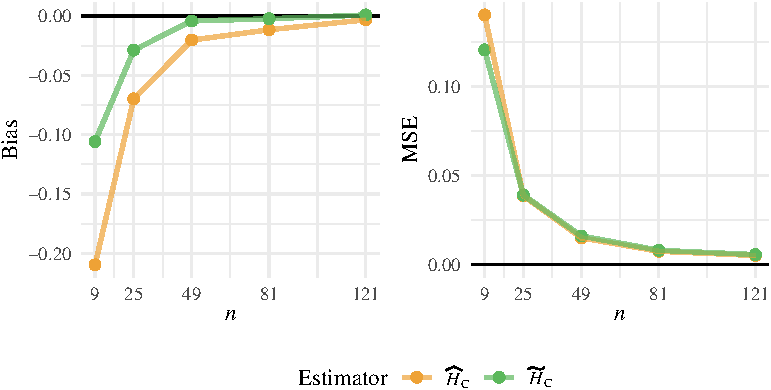
\includegraphics[width=\textwidth]{../../Figures/PDF/Plot_bias_mse_correa-1}
    \caption{}
    \label{fig:subfig4}
  \end{subfigure}
	\begin{subfigure}[t]{0.48\textwidth}
    \centering
    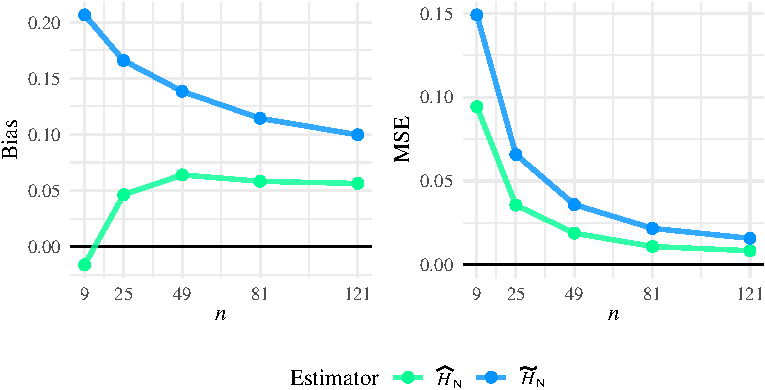
\includegraphics[width=\textwidth]{../../Figures/PDF/Plot_bias_mse_noughabi-1}
    \caption{}
    \label{fig:subfig5}
  \end{subfigure}
  \hfill
  \begin{subfigure}[t]{0.48\textwidth}
    \centering
    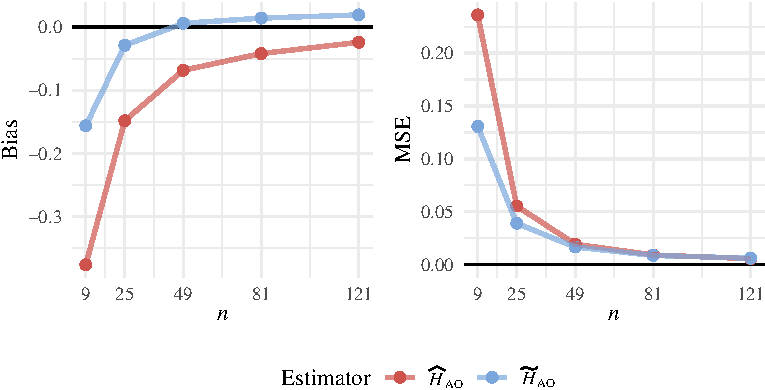
\includegraphics[width=\textwidth]{../../Figures/PDF/Plot_bias_mse_AO-1}
    \caption{}
    \label{fig:subfig6}
  \end{subfigure}
  \caption{Comparing Bias and MSE: original vs. bootstrap estimators, with, $\mu=1$ and $L=5$.}
  \label{fig:all_estimator}
\end{figure}

%I want to write as Fig. \ref{fig:all_estimator} \ref{fig:Firstfigure}--\ref{fig:subfig6}.
Based on previous simulations, the bootstrap technique did not improve the \(\widetilde{H}_{\text{NA}}\) estimator. 
This might occur because the original estimator overestimates the entropy values, showing a positive bias. 
This tendency to overestimate persists with the use of bootstrap, contributing to an increase in bias and MSE.

However, the improvement observed in the most estimators with the application of bootstrap techniques is notable, especially for sample sizes below 81. 
This performance is superior for the \(\widetilde{H}_{\text{C}}\), \(\widetilde{H}_{\text{E}}\), and \(\widetilde{H}_{\text{AO}}\) estimators. 
Therefore, we proceed to perform a comparison of bias and MSE of these three estimators alongside with their original versions, with \(1000\) samples from the \(\Gamma_{\text{SAR}}\) distribution of
size \(n\in\left\{9, 25, 49, 81, 121\right\}\), with \(\mu\in\left\{1, 10\right\}\), \(L=5\), and \(B=200\) bootstrap samples, as shown in Figure~\ref{fig:Plot_bias_mse_gi0} and Table~\ref{tab:table_final}.

%\begin{figure}[htb]
%{\centering 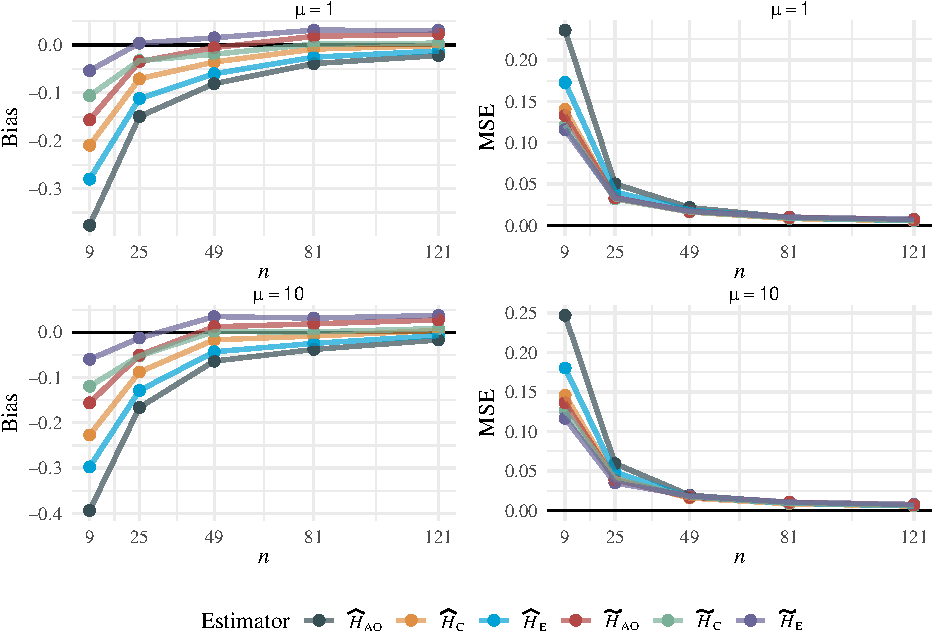
\includegraphics[width=0.7\linewidth]{../../Figures/PDF/Plot_bias_mse_gi0-2}
%}
%\caption{Bias and MSE of the entropy estimators for the $\Gamma_{\text{SAR}}$, with $L=5$.}\label{fig:Plot_bias_mse_gi0}
%\end{figure}
\begin{figure}[htb]
{\centering 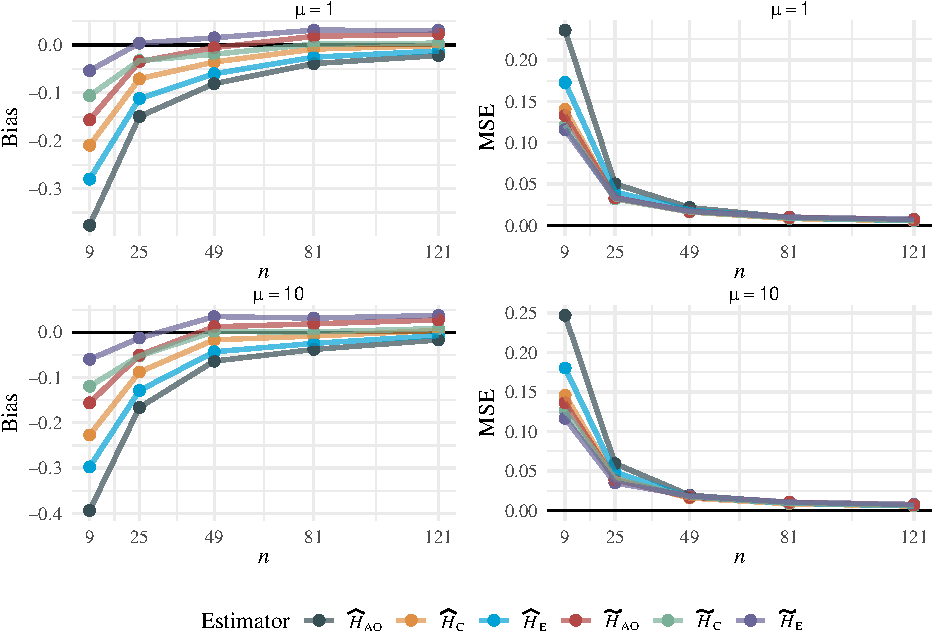
\includegraphics[width=0.8\linewidth]{../../Figures/PDF/Plot_bias_mse_gi0-2} 

}
\caption{Bias and MSE of the entropy estimators for the $\Gamma_{\text{SAR}}$, with $L=5$.}\label{fig:Plot_bias_mse_gi0}
\end{figure}


\setlength{\tabcolsep}{6pt}
\begin{table}[H]
\centering
\caption{\label{tab:table_final}Bias and MSE of the entropy estimators for the $\Gamma_{\text{SAR}}$, with $L=5$.}
\resizebox{\ifdim\width>\linewidth\linewidth\else\width\fi}{!}{
\begin{tabular}[t]{crllllllllllll}
\toprule
\multicolumn{1}{c}{ } & \multicolumn{1}{c}{ } & \multicolumn{6}{c}{Bias} & \multicolumn{6}{c}{MSE} \\
\cmidrule(l{3pt}r{3pt}){3-8} \cmidrule(l{3pt}r{3pt}){9-14}
\multicolumn{1}{r}{$\bm{\mu}$} & \multicolumn{1}{r}{$\bm{n}$} & \multicolumn{1}{r}{$\bm{\widehat{H}_{\text{C}}}$} & \multicolumn{1}{r}{$\bm{\widehat{H}_{\text{E}}}$} & \multicolumn{1}{r}{$\bm{\widehat{H}_{\text{AO}}}$} & \multicolumn{1}{r}{$\bm{\widetilde{H}_{\text{C}}}$} & \multicolumn{1}{r}{$\bm{\widetilde{H}_{\text{E}}}$} & \multicolumn{1}{r}{$\bm{\widetilde{H}_{\text{AO}}}$} & \multicolumn{1}{r}{$\bm{\widehat{H}_{\text{C}}}$} & \multicolumn{1}{r}{$\bm{\widehat{H}_{\text{E}}}$} & \multicolumn{1}{r}{$\bm{\widehat{H}_{\text{AO}}}$} & \multicolumn{1}{r}{$\bm{\widetilde{H}_{\text{C}}}$} & \multicolumn{1}{r}{$\bm{\widetilde{H}_{\text{E}}}$} & \multicolumn{1}{r}{$\bm{\widetilde{H}_{\text{AO}}}$}\\
\midrule
 & $9$ & $-0.210$ & $-0.280$ & $-0.377$ & $-0.106$ & $-0.054$ & $-0.156$ & $\phantom{-}0.140$ & $\phantom{-}0.173$ & $\phantom{-}0.236$ & $\phantom{-}0.121$ & $\phantom{-}0.116$ & $\phantom{-}0.133$\\

 & $25$ & $-0.071$ & $-0.112$ & $-0.149$ & $-0.033$ & $\phantom{-}0.004$ & $-0.035$ & $\phantom{-}0.032$ & $\phantom{-}0.040$ & $\phantom{-}0.050$ & $\phantom{-}0.032$ & $\phantom{-}0.033$ & $\phantom{-}0.033$\\

 & $49$ & $-0.036$ & $-0.060$ & $-0.081$ & $-0.020$ & $\phantom{-}0.015$ & $-0.006$ & $\phantom{-}0.016$ & $\phantom{-}0.019$ & $\phantom{-}0.021$ & $\phantom{-}0.016$ & $\phantom{-}0.017$ & $\phantom{-}0.017$\\

 & $81$ & $-0.009$ & $-0.026$ & $-0.039$ & $\phantom{-}0.002$ & $\phantom{-}0.031$ & $\phantom{-}0.018$ & $\phantom{-}0.008$ & $\phantom{-}0.009$ & $\phantom{-}0.010$ & $\phantom{-}0.009$ & $\phantom{-}0.010$ & $\phantom{-}0.009$\\

\multirow{-5}{*}[2\dimexpr\aboverulesep+\belowrulesep+\cmidrulewidth]{\centering\arraybackslash 1} & $121$ & $-0.001$ & $-0.013$ & $-0.022$ & $\phantom{-}0.004$ & $\phantom{-}0.030$ & $\phantom{-}0.023$ & $\phantom{-}0.005$ & $\phantom{-}0.006$ & $\phantom{-}0.006$ & $\phantom{-}0.006$ & $\phantom{-}0.007$ & $\phantom{-}0.007$\\
\cmidrule{1-14}
 & $9$ & $-0.227$ & $-0.297$ & $-0.394$ & $-0.119$ & $-0.060$ & $-0.156$ & $\phantom{-}0.146$ & $\phantom{-}0.180$ & $\phantom{-}0.247$ & $\phantom{-}0.126$ & $\phantom{-}0.117$ & $\phantom{-}0.136$\\

 & $25$ & $-0.088$ & $-0.129$ & $-0.166$ & $-0.052$ & $-0.013$ & $-0.050$ & $\phantom{-}0.040$ & $\phantom{-}0.048$ & $\phantom{-}0.059$ & $\phantom{-}0.040$ & $\phantom{-}0.035$ & $\phantom{-}0.039$\\

 & $49$ & $-0.017$ & $-0.043$ & $-0.064$ & $\phantom{-}0.001$ & $\phantom{-}0.035$ & $\phantom{-}0.012$ & $\phantom{-}0.016$ & $\phantom{-}0.017$ & $\phantom{-}0.019$ & $\phantom{-}0.018$ & $\phantom{-}0.019$ & $\phantom{-}0.017$\\

 & $81$ & $-0.008$ & $-0.025$ & $-0.038$ & $\phantom{-}0.001$ & $\phantom{-}0.031$ & $\phantom{-}0.019$ & $\phantom{-}0.009$ & $\phantom{-}0.009$ & $\phantom{-}0.010$ & $\phantom{-}0.009$ & $\phantom{-}0.011$ & $\phantom{-}0.010$\\

\multirow{-5}{*}[2\dimexpr\aboverulesep+\belowrulesep+\cmidrulewidth]{\centering\arraybackslash 10} & $121$ & $\phantom{-}0.004$ & $-0.007$ & $-0.017$ & $\phantom{-}0.008$ & $\phantom{-}0.037$ & $\phantom{-}0.027$ & $\phantom{-}0.006$ & $\phantom{-}0.006$ & $\phantom{-}0.006$ & $\phantom{-}0.006$ & $\phantom{-}0.008$ & $\phantom{-}0.007$\\
\bottomrule
\end{tabular}}
\end{table}

\section{Coefficient of variation and a robust
alternative}\label{coefficient-of-variation-and-a-robust-alternative}

The population CV is defined as a ratio of the population standard
deviation \((\sigma)\) to the population mean \((\mu)\): 
\begin{align}
    \text{CV}=\frac{\sigma}{\mu}, \quad \mu \neq 0.
\end{align}

We explore a robust alternative to CV, as described
in~\citep{Ospina2019}, which incorporates the ratio between the mean
absolute deviation from the median (MnAD) and the median, two well-known
robust measures of scale and location, respectively. 
The sample version for the MnAD is defined as \(n^{-1}\sum_{i=1}^n|x_i-\widehat{Q}_2|\),
where \(\widehat{Q}_2\) is an estimate for the median of the population,
which can be approximated by the median of the sample.

\section{Hypothesis Testing}\label{sec:test}

We aim to test the following hypotheses: \[
\begin{cases}
  \mathcal{H}_0: \text{ The data come from the } \Gamma_{\text{SAR}}\text{ law},\\ 
  \mathcal{H}_1:\text{ The data come from the } G_I^0 \text{ distribution}.
\end{cases}
\] We are testing the hypothesis that the data are fully-developed
speckle versus the alternative of data with roughness. As for the
parametric problem, once it is not possible to define the hypothesis
\(\mathcal{H}_0=\alpha=-\infty\), it is impossible to solve this problem
with parametric inference alternatives (such as likelihood ratio, score,
gradient, and Wald hypothesis test). The proposed tests to solve this
physical problem in SAR systems are described below.

\subsection{The Proposed Test Based on Non-parametric
Entropy}\label{the-proposed-test-based-on-non-parametric-entropy}

For a random sample \(\bm{Z}=(Z_1, Z_2,\ldots,Z_n)\) from a distribution
\(\mathcal{D}\), a test statistic is proposed. It is based on an
empirical distribution that arises from the difference between
non-parametrically estimated entropies \(\widetilde{H}(\bm{Z})\) and the
analytical entropy of \(\Gamma_{\text{SAR}}\)~\eqref{E:E-gamma}
evaluated at the logarithm of the sample mean, where \(L\geq 1\) is
known.

Hence, the entropy-based test statistic is defined as: \begin{equation}
\label{Eq:test_e}
S(\bm{Z};L)= \widetilde{H}(\bm{Z})-\left[H_{\Gamma_{\text{SAR}}}(L)+\ln \overline{\bm{Z}}\right].
\end{equation}

This test statistic aims to assess the behavior of the data under the
null hypothesis using the empirical distribution. If the data represent
fully-developed speckle, the density should center around zero, i.e.,
\(S(\bm{Z};L)\approx 0\). Otherwise, the empirical distribution would
shift from zero under the alternative hypothesis, suggesting significant
differences and heterogeneous clutter.

The comparison between the bootstrap-improved estimators is shown in
Table~\ref{tab:table_time}, where the test accuracy under the null
hypothesis is presented alongside running times. The test accuracy is
evaluated through 1000 simulated samples of different sizes, with each
size replicated 100 times using bootstrap resampling.

The processing time is an important feature, especially considering the
application of these estimators to large datasets of SAR images, as seen
in Chapter~\ref{chp:results}.
\setlength{\tabcolsep}{7pt}
\begin{table}[htb]
\centering\centering
\caption{\label{tab:table_time}Test accuracy and processing time for each bootstrap-improved estimator. }
\resizebox{\ifdim\width>\linewidth\linewidth\else\width\fi}{!}{
\small
\begin{tabu} to \linewidth {>{\centering}X>{\centering}X>{\centering}X>{\centering}X>{\centering}X}
\toprule
\multicolumn{1}{c}{\textbf{Estimator}} & \multicolumn{1}{c}{$\bm{L}$} & \multicolumn{1}{c}{$\bm{n}$} & \multicolumn{1}{c}{$S(\bm{Z}; L)$} & \multicolumn{1}{c}{\textbf{ Time} (s)}\\
\midrule
 &  & $25$ & $-0.00152$ & 22.53\\

 &  & $49$ & $\phantom{-}0.00515$ & 40.35\\

 &  & $81$ & $\phantom{-}0.00625$ & 63.93\\

 & \multirow{-4}{*}[1.5\dimexpr\aboverulesep+\belowrulesep+\cmidrulewidth]{\centering\arraybackslash $2$} & $121$ & $\phantom{-}0.00751$ & 97.06\\

\cline{3-5}
 &  & $25$ & $-0.04332$ & 22.25\\

 &  & $49$ & $-0.01659$ & 33.42\\

 &  & $81$ & $-0.00393$ & 50.94\\

\multirow{-8}{*}[3.5\dimexpr\aboverulesep+\belowrulesep+\cmidrulewidth]{\centering\arraybackslash $\widetilde{H}_{\text{C}}$} & \multirow{-4}{*}[1.5\dimexpr\aboverulesep+\belowrulesep+\cmidrulewidth]{\centering\arraybackslash $8$} & $121$ & $\phantom{-}0.00261$ & 97.35\\
\cmidrule{1-5}
 &  & $25$ & $\phantom{-}0.02204$ & 4.66\\

 &  & $49$ & $\phantom{-}0.03452$ & 5.55\\

 &  & $81$ & $\phantom{-}0.03195$ & 6.89\\

 & \multirow{-4}{*}[1.5\dimexpr\aboverulesep+\belowrulesep+\cmidrulewidth]{\centering\arraybackslash $2$} & $121$ & $\phantom{-}0.03012$ & 7.90\\

\cline{3-5}
 &  & $25$ & $\phantom{-}0.00801$ & 4.81\\

 &  & $49$ & $\phantom{-}0.01654$ & 5.43\\

 &  & $81$ & $\phantom{-}0.03036$ & 6.38\\

\multirow{-8}{*}[3.5\dimexpr\aboverulesep+\belowrulesep+\cmidrulewidth]{\centering\arraybackslash $\widetilde{H}_{\text{E}}$} & \multirow{-4}{*}[1.5\dimexpr\aboverulesep+\belowrulesep+\cmidrulewidth]{\centering\arraybackslash $8$} & $121$ & $\phantom{-}0.03137$ & 7.46\\
\cmidrule{1-5}
 &  & $25$ & $-0.01935$ & 4.61\\

 &  & $49$ & $\phantom{-}0.00786$ & 5.19\\

 &  & $81$ & $\phantom{-}0.01995$ & 6.70\\

 & \multirow{-4}{*}[1.5\dimexpr\aboverulesep+\belowrulesep+\cmidrulewidth]{\centering\arraybackslash $2$} & $121$ & $\phantom{-}0.01741$ & 7.41\\

\cline{3-5}
 &  & $25$ & $-0.04020$ & 4.74\\

 &  & $49$ & $\phantom{-}0.00047$ & 5.35\\

 &  & $81$ & $\phantom{-}0.01176$ & 6.21\\

\multirow{-8}{*}[3.5\dimexpr\aboverulesep+\belowrulesep+\cmidrulewidth]{\centering\arraybackslash $\widetilde{H}_{\text{AO}}$} & \multirow{-4}{*}[1.5\dimexpr\aboverulesep+\belowrulesep+\cmidrulewidth]{\centering\arraybackslash $8$} & $121$ & $\phantom{-}0.02019$ & 7.48\\
\bottomrule
\end{tabu}}
\end{table}

As visible from Table~\ref{tab:table_time}, the accuracy of the test
results across the three estimators shows similarities in specific
sample sizes. 
However, practical scenarios in SAR image processing often
involve small sample sizes, typically obtained over windows of size
\(7\times7\).\\
It is also noteworthy that the \(\widetilde{H}_{\text{AO}}\) estimator
exhibited the shortest processing time, followed by
\(\widetilde{H}_{\text{E}}\) and \(\widetilde{H}_{\text{C}}\).
Considering this aspect, we select the \(\widetilde{H}_{\text{AO}}\)
estimator for subsequent simulations.
 Henceforth, the test statistical
~\eqref{Eq:test_e} will be denoted as:
\(S_{\widetilde{H}_{\text{AO}}}(\bm{Z}; L)\).

We now verify the normality of the data generated by the
\(S_{\widetilde{H}_{\text{AO}}}(\bm{Z}; L)\) test.
Figure~\ref{fig:Plot_density} shows the empirical densities obtained by
applying the \(S_{\widetilde{H}_{\text{AO}}}(\bm{Z}; L)\) test to
different sample sizes drawn from the \(\Gamma_{\text{SAR}}\)
distribution, where \(L\) takes values \(\left\{3,5, 8,11\right\}\) and
\(\mu=1\). 
\begin{figure}[htb]

{\centering 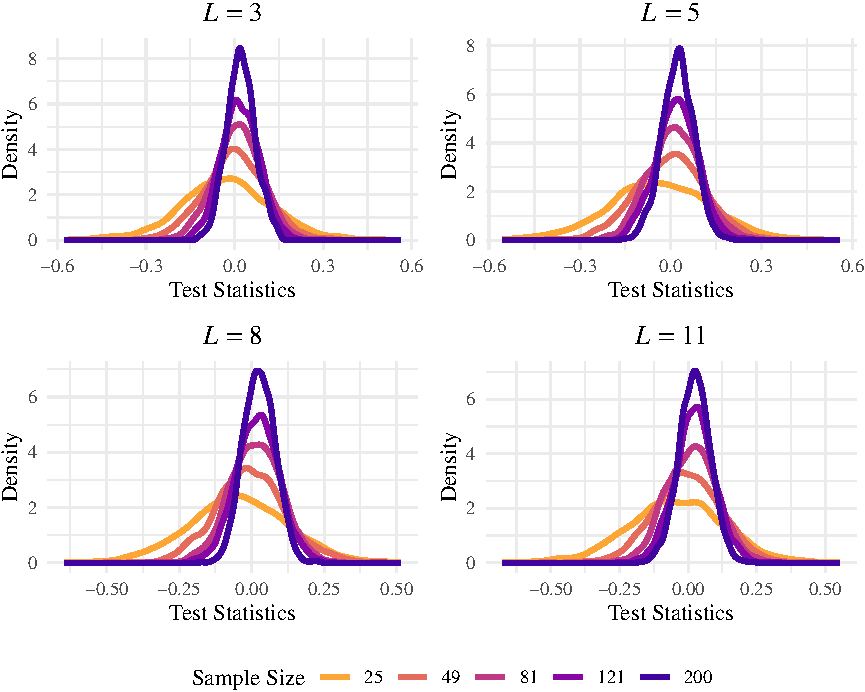
\includegraphics[width=0.8\linewidth]{../../Figures/PDF/Plot_density-1} 

}

\caption{Empirical densities obtained from $S_{\widetilde{H}_{\text{AO}}}(\bm{Z}; L)$ test under the null hypothesis.}\label{fig:Plot_density}
\end{figure}

Additionally, Table~\ref{tab:table_stat_combined} summarizes
the main descriptive statistics, including mean, standard
deviation~(SD), variance~(Var), skewness~(SK), excessive kurtosis~(EK)
and Anderson--Darling \(p\) values for normality. 


\setlength{\tabcolsep}{5pt}
\begin{table}[H]
\centering\centering\centering
\caption{\label{tab:table_stat_combined}Descriptive analysis of $S_{\widetilde{H}_{\text{AO}}}(\bm{Z}; L)$, with $L\in\left\{3,5, 8,11\right\}$ and $\mu=1$.}
\resizebox{\ifdim\width>\linewidth\linewidth\else\width\fi}{!}{
\footnotesize
\begin{tabu} to \linewidth {>{\centering}X>{\centering}X>{\raggedleft}X>{\raggedleft}X>{\raggedleft}X>{\raggedleft}X>{\raggedleft}X>{\raggedleft}X}
\toprule
\multicolumn{1}{c}{$\bm{L}$} & \multicolumn{1}{c}{$\bm{n}$} & \multicolumn{1}{c}{\textbf{Mean}} & \multicolumn{1}{c}{\textbf{SD}} & \multicolumn{1}{c}{\textbf{Var}} & \multicolumn{1}{c}{\textbf{SK}} & \multicolumn{1}{c}{\textbf{EK}} & \multicolumn{1}{c}{$p$-\textbf{value}}\\
\midrule
 & $25$ & $-0.0280$ & $\phantom{-}0.1547$ & $\phantom{-}0.0239$ & $-0.0076$ & $\phantom{-}0.4734$ & $\phantom{-}0.0022$\\

 & $49$ & $-0.0003$ & $\phantom{-}0.1053$ & $\phantom{-}0.0111$ & $-0.0562$ & $\phantom{-}0.2610$ & $\phantom{-}0.0582$\\

 & $81$ & $\phantom{-}0.0124$ & $\phantom{-}0.0796$ & $\phantom{-}0.0063$ & $-0.0124$ & $\phantom{-}0.0536$ & $\phantom{-}0.5278$\\

 & $121$ & $\phantom{-}0.0187$ & $\phantom{-}0.0630$ & $\phantom{-}0.0040$ & $\phantom{-}0.0337$ & $-0.1826$ & $\phantom{-}0.5894$\\

\multirow{-5}{*}[2\dimexpr\aboverulesep+\belowrulesep+\cmidrulewidth]{\centering\arraybackslash 3} & $200$ & $\phantom{-}0.0215$ & $\phantom{-}0.0490$ & $\phantom{-}0.0024$ & $\phantom{-}0.0625$ & $-0.0473$ & $\phantom{-}0.0860$\\
\cmidrule{1-8}
 & $25$ & $-0.0379$ & $\phantom{-}0.1669$ & $\phantom{-}0.0278$ & $\phantom{-}0.0007$ & $\phantom{-}0.1420$ & $\phantom{-}0.3267$\\

 & $49$ & $-0.0015$ & $\phantom{-}0.1150$ & $\phantom{-}0.0132$ & $-0.1025$ & $\phantom{-}0.1998$ & $\phantom{-}0.2582$\\

 & $81$ & $\phantom{-}0.0145$ & $\phantom{-}0.0869$ & $\phantom{-}0.0075$ & $\phantom{-}0.1008$ & $\phantom{-}0.5297$ & $\phantom{-}0.1121$\\

 & $121$ & $\phantom{-}0.0198$ & $\phantom{-}0.0687$ & $\phantom{-}0.0047$ & $\phantom{-}0.0127$ & $\phantom{-}0.0222$ & $\phantom{-}0.2919$\\

\multirow{-5}{*}[2\dimexpr\aboverulesep+\belowrulesep+\cmidrulewidth]{\centering\arraybackslash 5} & $200$ & $\phantom{-}0.0236$ & $\phantom{-}0.0529$ & $\phantom{-}0.0028$ & $-0.0467$ & $\phantom{-}0.0977$ & $\phantom{-}0.3346$\\
\cmidrule{1-8}
 & $25$ & $-0.0464$ & $\phantom{-}0.1680$ & $\phantom{-}0.0282$ & $-0.0121$ & $\phantom{-}0.0980$ & $\phantom{-}0.6477$\\

 & $49$ & $-0.0031$ & $\phantom{-}0.1202$ & $\phantom{-}0.0144$ & $\phantom{-}0.1282$ & $\phantom{-}0.2000$ & $\phantom{-}0.0038$\\

 & $81$ & $\phantom{-}0.0137$ & $\phantom{-}0.0883$ & $\phantom{-}0.0078$ & $-0.0279$ & $\phantom{-}0.2554$ & $\phantom{-}0.5567$\\

 & $121$ & $\phantom{-}0.0200$ & $\phantom{-}0.0738$ & $\phantom{-}0.0055$ & $-0.0089$ & $\phantom{-}0.0686$ & $\phantom{-}0.7502$\\

\multirow{-5}{*}[2\dimexpr\aboverulesep+\belowrulesep+\cmidrulewidth]{\centering\arraybackslash 8} & $200$ & $\phantom{-}0.0260$ & $\phantom{-}0.0546$ & $\phantom{-}0.0030$ & $\phantom{-}0.0716$ & $-0.0349$ & $\phantom{-}0.3771$\\
\cmidrule{1-8}
 & $25$ & $-0.0442$ & $\phantom{-}0.1735$ & $\phantom{-}0.0301$ & $-0.1422$ & $\phantom{-}0.2413$ & $\phantom{-}0.0981$\\

 & $49$ & $-0.0019$ & $\phantom{-}0.1201$ & $\phantom{-}0.0144$ & $-0.0503$ & $\phantom{-}0.1464$ & $\phantom{-}0.9576$\\

 & $81$ & $\phantom{-}0.0127$ & $\phantom{-}0.0917$ & $\phantom{-}0.0084$ & $-0.0172$ & $\phantom{-}0.0333$ & $\phantom{-}0.3179$\\

 & $121$ & $\phantom{-}0.0239$ & $\phantom{-}0.0729$ & $\phantom{-}0.0053$ & $-0.0127$ & $\phantom{-}0.2102$ & $\phantom{-}0.0596$\\

\multirow{-5}{*}[2\dimexpr\aboverulesep+\belowrulesep+\cmidrulewidth]{\centering\arraybackslash 11} & $200$ & $\phantom{-}0.0234$ & $\phantom{-}0.0572$ & $\phantom{-}0.0033$ & $-0.0233$ & $\phantom{-}0.1072$ & $\phantom{-}0.6740$\\
\bottomrule
\end{tabu}}
\end{table}
Results with \(p\) values greater than \(0.05\) do not indicate a violation of the
normality assumption. 
A low variance, skewness, and excessive kurtosis
of almost zero indicate limited dispersion, asymmetry, and a light tail.

Normal Q--Q plots confirm no evidence against a normal distribution, as
shown in Figure~\ref{fig:Plot_normality_qq}.
\begin{figure}[H]
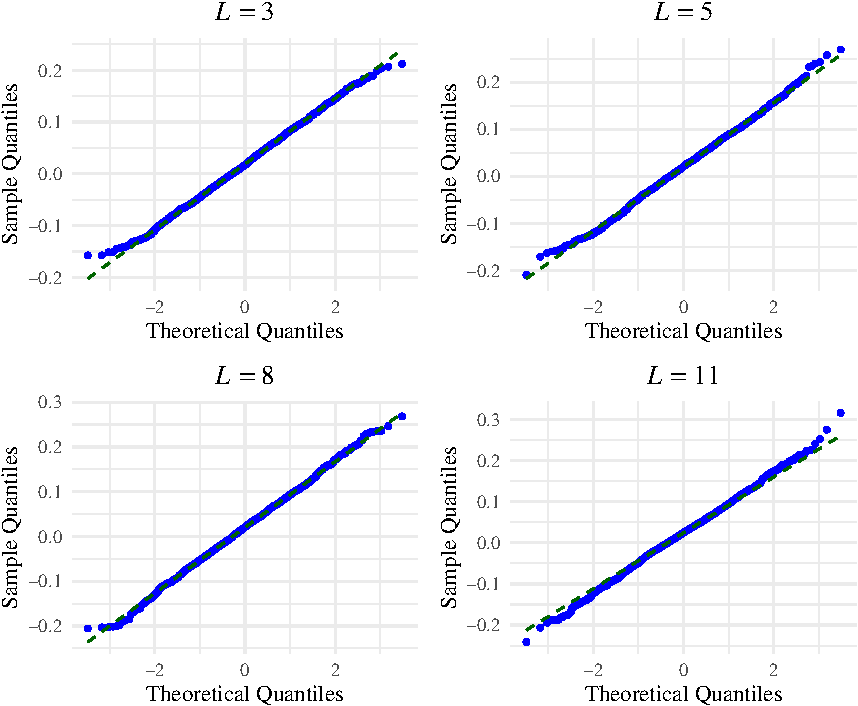
\includegraphics[width=0.9\linewidth]{../../Figures/PDF/Plot_normality_qq-1} \caption{Normal Q--Q plots for  $n=121$.}\label{fig:Plot_normality_qq}
\end{figure}

After checking the data's normality, we examined the proposed test's
abilities in terms of size and power. Under \(\mathcal{H}_0\), the
distribution of the test statistic is asymptotically normal. Therefore,
the \(p\) values are calculated as \(2\Phi(-|\varepsilon|)\), where
\(\Phi\) is the standard Gaussian cumulative distribution function, and
\(\varepsilon\) is the standardized test statistic given by: \[
\varepsilon=\frac{\widetilde{H}_{\text{AO}}(\bm{Z})-\left[H_{\Gamma_{\text{SAR}}}(L)+\ln \overline{\bm{Z}}\right]}{\widehat\sigma}.
\]

We have nominal levels of \SI{1}{\percent}, \SI{5}{\percent}, and
\SI{10}{\percent}. In terms of size, \(1000\) simulations were used for
different sample sizes from the \(\Gamma_{\text{SAR}}\) distribution,
with varying values of \(L\), and \(\mu=1\). In all cases, the nominal
level was achieved. We assessed the test power using \(1000\)
simulations for different sample sizes from the \(G_I^0\) distribution,
with \(\mu=1\), and \(\alpha=-2\). The power generally improves with
increasing sample size and number of looks. The results are shown in
Table~\ref{tab:table_size_power}.

\begin{table}[htb]
\centering\centering
\caption{\label{tab:table_size_power}Size and Power of the $S_{\widetilde{H}_{\text{AO}}}(\bm{Z})$ test statistic.}
\resizebox{\ifdim\width>\linewidth\linewidth\else\width\fi}{!}{
\begin{tabu} to \linewidth {>{\centering}X>{\centering}X>{\centering}X>{\centering}X>{\centering}X>{\centering}X>{\centering}X>{\centering}X}
\toprule
\multicolumn{1}{c}{ } & \multicolumn{1}{c}{ } & \multicolumn{3}{c}{Size} & \multicolumn{3}{c}{Power} \\
\cmidrule(l{3pt}r{3pt}){3-5} \cmidrule(l{3pt}r{3pt}){6-8}
\multicolumn{1}{c}{$\bm{L}$} & \multicolumn{1}{c}{$\bm{n}$} & \multicolumn{1}{c}{$\bm{1\%}$} & \multicolumn{1}{c}{$\bm{5\%}$} & \multicolumn{1}{c}{$\bm{10\%}$} & \multicolumn{1}{c}{$\bm{1\%}$} & \multicolumn{1}{c}{$\bm{5\%}$} & \multicolumn{1}{c}{$\bm{10\%}$}\\
\midrule
 & 25 & $\phantom{-}0.0160$ & $\phantom{-}0.0620$ & $\phantom{-}0.1070$ & $\phantom{-}0.6900$ & $\phantom{-}0.8450$ & $\phantom{-}0.8340$\\

 & 49 & $\phantom{-}0.0100$ & $\phantom{-}0.0480$ & $\phantom{-}0.0960$ & $\phantom{-}0.6890$ & $\phantom{-}0.8920$ & $\phantom{-}0.8480$\\

 & 81 & $\phantom{-}0.0120$ & $\phantom{-}0.0490$ & $\phantom{-}0.1080$ & $\phantom{-}0.6260$ & $\phantom{-}0.8750$ & $\phantom{-}0.8540$\\

\multirow{-4}{*}[1.5\dimexpr\aboverulesep+\belowrulesep+\cmidrulewidth]{\centering\arraybackslash 3} & 121 & $\phantom{-}0.0090$ & $\phantom{-}0.0690$ & $\phantom{-}0.1190$ & $\phantom{-}0.5680$ & $\phantom{-}0.8620$ & $\phantom{-}0.8230$\\
\cmidrule{1-8}
 & 25 & $\phantom{-}0.0210$ & $\phantom{-}0.0660$ & $\phantom{-}0.1130$ & $\phantom{-}0.9120$ & $\phantom{-}0.9620$ & $\phantom{-}0.9880$\\

 & 49 & $\phantom{-}0.0100$ & $\phantom{-}0.0460$ & $\phantom{-}0.1080$ & $\phantom{-}0.9470$ & $\phantom{-}0.9820$ & $\phantom{-}0.9960$\\

 & 81 & $\phantom{-}0.0120$ & $\phantom{-}0.0560$ & $\phantom{-}0.1070$ & $\phantom{-}0.9580$ & $\phantom{-}0.9900$ & $\phantom{-}0.9960$\\

\multirow{-4}{*}[1.5\dimexpr\aboverulesep+\belowrulesep+\cmidrulewidth]{\centering\arraybackslash 5} & 121 & $\phantom{-}0.0150$ & $\phantom{-}0.0640$ & $\phantom{-}0.1150$ & $\phantom{-}0.9420$ & $\phantom{-}0.9780$ & $\phantom{-}0.9950$\\
\cmidrule{1-8}
 & 25 & $\phantom{-}0.0210$ & $\phantom{-}0.0650$ & $\phantom{-}0.1080$ & $\phantom{-}0.9930$ & $\phantom{-}0.9950$ & $\phantom{-}0.9970$\\

 & 49 & $\phantom{-}0.0060$ & $\phantom{-}0.0470$ & $\phantom{-}0.0860$ & $\phantom{-}0.9980$ & $\phantom{-}1.0000$ & $\phantom{-}0.9970$\\

 & 81 & $\phantom{-}0.0120$ & $\phantom{-}0.0490$ & $\phantom{-}0.1000$ & $\phantom{-}0.9930$ & $\phantom{-}0.9980$ & $\phantom{-}0.9990$\\

\multirow{-4}{*}[1.5\dimexpr\aboverulesep+\belowrulesep+\cmidrulewidth]{\centering\arraybackslash 8} & 121 & $\phantom{-}0.0150$ & $\phantom{-}0.0650$ & $\phantom{-}0.1220$ & $\phantom{-}0.9970$ & $\phantom{-}0.9990$ & $\phantom{-}0.9980$\\
\cmidrule{1-8}
 & 25 & $\phantom{-}0.0130$ & $\phantom{-}0.0610$ & $\phantom{-}0.1000$ & $\phantom{-}0.9990$ & $\phantom{-}0.9990$ & $\phantom{-}0.9990$\\

 & 49 & $\phantom{-}0.0100$ & $\phantom{-}0.0450$ & $\phantom{-}0.0920$ & $\phantom{-}0.9980$ & $\phantom{-}0.9990$ & $\phantom{-}0.9990$\\

 & 81 & $\phantom{-}0.0170$ & $\phantom{-}0.0530$ & $\phantom{-}0.1050$ & $\phantom{-}1.0000$ & $\phantom{-}1.0000$ & $\phantom{-}1.0000$\\

\multirow{-4}{*}[1.5\dimexpr\aboverulesep+\belowrulesep+\cmidrulewidth]{\centering\arraybackslash 11} & 121 & $\phantom{-}0.0160$ & $\phantom{-}0.0680$ & $\phantom{-}0.1180$ & $\phantom{-}0.9980$ & $\phantom{-}1.0000$ & $\phantom{-}0.9980$\\
\bottomrule
\end{tabu}}
\end{table}

\subsection{The Proposed Test Based on Coefficient of Variation and a
Robust
Alternative}\label{the-proposed-test-based-on-coefficient-of-variation-and-a-robust-alternative}

In addition to the \(S_{\widetilde{H}_{\text{AO}}}(\bm{Z}; L)\) test, we
also propose a test statistic based on the classical CV. This test
statistic is defined as follows: \begin{align}
    T_{\text{CV}}=\frac{S}{\overline{Z}},
\end{align} where \(S\) and \(\overline{Z}\) are the sample standard
deviation and mean, respectively.

Similarly, we use another test statistic based on the ratio of the MnAD
to the median. This statistic is given by: \begin{align}
    T_{\text{CV}_{\text{MnAD}}}=\frac{\text{MnAD}}{\text{Median}}.
\end{align}

We proceed to identify suitable models for these estimators of the CV,
and then form test statistics.

The situations in which the use of CV and \(\text{CV}_{\text{MnAD}}\)
may be appropriate, i.e., when the observations are positive, the
log-normal (LN) and the inverse Gaussian distribution (IG) are often
more appropriate than the Gamma and Weibull
distributions~\citep{Chaubey2017,takagi1997application}.

It is shown that the IG distribution is well approximated by the
log-normal distribution, which means that the IG distribution also does
not share the problem of the non-existence of a fixed-width confidence
interval with the Gaussian case~\citep{whitmore1978}.

The biparametric LN distribution has density:

\begin{align}
    f_Z(z;\mu_{\text{LN}}, \sigma_{\text{LN}} )=\frac{1}{\sigma_{\text{LN}} z\sqrt{2\pi}}\exp\left\{-\frac{(\ln z- \mu_{\text{LN}})^2}{2\sigma_{\text{LN}}^2}\right\}\mathbbm 1_{\mathbbm R_+}(z),
\end{align}\\
with \(\mu_{\text{LN}}\) is any real number, and \(\sigma_{\text{LN}}\)
is positive.

\subsection{Model Selection Criterion}\label{model-selection-criterion}

We used the Akaike information criterion (AIC) and the Bayesian
information criterion (BIC) to select the best-fitting distribution.

The AIC deals with the trade-off between the goodness-of-fit and the
model's simplicity in terms of the number of model
parameters~\citep{Burnham2004}. The model or distribution with the lowest
value of AIC is chosen to be the best. The BIC assesses goodness-of-fit
of a distribution or model, but avoids overfitting by penalising
additional degrees of freedom~\citep{Dziak2019}. The model with the
lowest BIC value is chosen as the best.

The AIC and BIC results in
Tables~\ref{tab:table_aic_gamma}--\ref{tab:table_aic_gio_MnADmedian}
indicate that the CV and \(\text{CV}_{\text{MnAD}}\) data from different
distributed \(\Gamma_{\text{SAR}}\) and \(G_I^0\) synthetic sample sizes
match the properties of an LN distribution. It is important to note that
this conclusion was drawn empirically based on a dictionary of
analytically tractable distributions and well-defined under
biparametric, unimodal, asymmetric, and positive distributions.

Figures~\ref{fig:Plot_cv}--\ref{fig:Plot_madmed_gi0_MnADmedian} show
empirical and fitted density plots, Q--Q plots, P--P plots, as well as
empirical and fitted cumulative distribution functions. They provide
qualitative sources that confirm that the LN distribution is the most
appropriate distribution. As expected, both test statistics work well
under the null hypothesis. Under the alternative hypothesis, the P--P
plot shows that \(\text{CV}_{\text{MnAD}}\) is more robust than CV,
although both statistics suffer from the tail effect caused by the
distributed \(G_I^0\) data.

\begin{table}[H]
\centering\centering
\caption{\label{tab:table_aic_gamma}AIC and BIC values for evaluating the best distribution with CV data from $\Gamma_{\text{SAR}}$.}
\resizebox{\ifdim\width>\linewidth\linewidth\else\width\fi}{!}{
\begin{tabu} to \linewidth {>{\centering}X>{\centering}X>{\centering}X>{\centering}X>{\raggedleft}X>{\raggedleft}X>{\raggedleft}X}
\toprule
\multicolumn{1}{c}{\textbf{Criterion}} & \multicolumn{1}{c}{$\bm{n}$} & \multicolumn{1}{c}{\textbf{Normal}} & \multicolumn{1}{c}{\textbf{Lognormal}} & \multicolumn{1}{c}{\textbf{Gamma}} & \multicolumn{1}{c}{\textbf{Weibull}} & \multicolumn{1}{c}{\textbf{Inverse Gaussian}}\\
\midrule
 & $25$ & $-38031.9$ & $-38266.7$ & $-38311.8$ & $-36413.2$ & $-38261.6$\\

 & $49$ & $-47698.2$ & $-47913.7$ & $-47905.6$ & $-45554.0$ & $-47911.6$\\

 & $81$ & $-55382.1$ & $-55494.7$ & $-55494.9$ & $-53220.4$ & $-55493.8$\\

\multirow{-4}{*}[1.5\dimexpr\aboverulesep+\belowrulesep+\cmidrulewidth]{\centering\arraybackslash AIC} & $121$ & $-61344.9$ & $-61470.8$ & $-61453.8$ & $-58876.0$ & $-61470.5$\\
\cmidrule{1-7}
 & $25$ & $-38016.7$ & $-38251.5$ & $-38296.6$ & $-36398.0$ & $-38246.4$\\

 & $49$ & $-47683.0$ & $-47898.5$ & $-47890.4$ & $-45538.7$ & $-47896.4$\\

 & $81$ & $-55366.9$ & $-55479.5$ & $-55479.6$ & $-53205.2$ & $-55478.6$\\

\multirow{-4}{*}[1.5\dimexpr\aboverulesep+\belowrulesep+\cmidrulewidth]{\centering\arraybackslash BIC} & $121$ & $-61329.7$ & $-61455.6$ & $-61438.6$ & $-58860.8$ & $-61455.2$\\
\bottomrule
\end{tabu}}
\end{table}

\begin{table}[H]
\centering\centering
\caption{\label{tab:table_aic}AIC and BIC values for evaluating the best distribution with CV data from $G_I^0$.}
\resizebox{\ifdim\width>\linewidth\linewidth\else\width\fi}{!}{
\begin{tabu} to \linewidth {>{\centering}X>{\centering}X>{\centering}X>{\centering}X>{\centering}X>{\centering}X>{\centering}X}
\toprule
\multicolumn{1}{c}{\textbf{Criterion}} & \multicolumn{1}{c}{$\bm{n}$} & \multicolumn{1}{c}{\textbf{Normal}} & \multicolumn{1}{c}{\textbf{Lognormal}} & \multicolumn{1}{c}{\textbf{Gamma}} & \multicolumn{1}{c}{\textbf{Weibull}} & \multicolumn{1}{c}{\textbf{Inverse Gaussian}}\\
\midrule
 & $25$ & $\phantom{-}8254.04$ & $\phantom{-}2186.31$ & $\phantom{-}3628.40$ & $\phantom{-}8383.58$ & $\phantom{-}2257.63$\\

 & $49$ & $\phantom{-}8821.79$ & $\phantom{-}1689.03$ & $\phantom{-}3483.10$ & $\phantom{-}9533.53$ & $\phantom{-}1835.29$\\

 & $81$ & $\phantom{-}8525.81$ & $\phantom{-}866.29$ & $\phantom{-}2853.31$ & $\phantom{-}9822.48$ & $\phantom{-}1057.91$\\

\multirow{-4}{*}[1.5\dimexpr\aboverulesep+\belowrulesep+\cmidrulewidth]{\centering\arraybackslash AIC} & $121$ & $\phantom{-}8708.81$ & $\phantom{-}131.86$ & $\phantom{-}2341.06$ & $\phantom{-}10506.49$ & $\phantom{-}398.53$\\
\cmidrule{1-7}
 & $25$ & $\phantom{-}8269.27$ & $\phantom{-}2201.54$ & $\phantom{-}3643.63$ & $\phantom{-}8398.81$ & $\phantom{-}2272.86$\\

 & $49$ & $\phantom{-}8837.02$ & $\phantom{-}1704.26$ & $\phantom{-}3498.33$ & $\phantom{-}9548.76$ & $\phantom{-}1850.52$\\

 & $81$ & $\phantom{-}8541.04$ & $\phantom{-}881.52$ & $\phantom{-}2868.55$ & $\phantom{-}9837.72$ & $\phantom{-}1073.14$\\

\multirow{-4}{*}[1.5\dimexpr\aboverulesep+\belowrulesep+\cmidrulewidth]{\centering\arraybackslash BIC} & $121$ & $\phantom{-}8724.04$ & $\phantom{-}147.09$ & $\phantom{-}2356.29$ & $\phantom{-}10521.72$ & $\phantom{-}413.76$\\
\bottomrule
\end{tabu}}
\end{table}

\begin{table}[H]
\centering\centering
\caption{\label{tab:table_aic_gamma_madmed}AIC and BIC values for evaluating the best distribution with $\text{CV}_{\text{MnAD}}$ data from $\Gamma_{\text{SAR}}$.}
\resizebox{\ifdim\width>\linewidth\linewidth\else\width\fi}{!}{
\begin{tabu} to \linewidth {>{\centering}X>{\centering}X>{\centering}X>{\centering}X>{\centering}X>{\centering}X>{\centering}X}
\toprule
\multicolumn{1}{c}{\textbf{Criterion}} & \multicolumn{1}{c}{$\bm{n}$} & \multicolumn{1}{c}{\textbf{Normal}} & \multicolumn{1}{c}{\textbf{Lognormal}} & \multicolumn{1}{c}{\textbf{Gamma}} & \multicolumn{1}{c}{\textbf{Weibull}} & \multicolumn{1}{c}{\textbf{Inverse Gaussian}}\\
\midrule
 & $25$ & $-38375.56$ & $-39147.85$ & $-39066.29$ & $-36652.49$ & $-39143.61$\\

 & $49$ & $-48386.11$ & $-48795.32$ & $-48745.48$ & $-46240.91$ & $-48793.83$\\

 & $81$ & $-56072.87$ & $-56322.32$ & $-56290.02$ & $-53836.04$ & $-56322.12$\\

\multirow{-4}{*}[1.5\dimexpr\aboverulesep+\belowrulesep+\cmidrulewidth]{\centering\arraybackslash AIC} & $121$ & $-62217.14$ & $-62394.77$ & $-62369.32$ & $-59861.80$ & $-62394.57$\\
\cmidrule{1-7}
 & $25$ & $-38360.32$ & $-39132.62$ & $-39051.05$ & $-36637.26$ & $-39128.38$\\

 & $49$ & $-48370.87$ & $-48780.09$ & $-48730.25$ & $-46225.67$ & $-48778.60$\\

 & $81$ & $-56057.64$ & $-56307.09$ & $-56274.79$ & $-53820.81$ & $-56306.89$\\

\multirow{-4}{*}[1.5\dimexpr\aboverulesep+\belowrulesep+\cmidrulewidth]{\centering\arraybackslash BIC} & $121$ & $-62201.91$ & $-62379.54$ & $-62354.09$ & $-59846.56$ & $-62379.33$\\
\bottomrule
\end{tabu}}
\end{table}

\begin{table}[H]
\centering\centering
\caption{\label{tab:table_aic_gio_MnADmedian}AIC and BIC values for evaluating the best distribution with $\text{CV}_{\text{MnAD}}$ data from $G_I^0$.}
\resizebox{\ifdim\width>\linewidth\linewidth\else\width\fi}{!}{
\begin{tabu} to \linewidth {>{\centering}X>{\centering}X>{\centering}X>{\centering}X>{\centering}X>{\centering}X>{\centering}X}
\toprule
\multicolumn{1}{c}{\textbf{Criterion}} & \multicolumn{1}{c}{$\bm{n}$} & \multicolumn{1}{c}{\textbf{Normal}} & \multicolumn{1}{c}{\textbf{Lognormal}} & \multicolumn{1}{c}{\textbf{Gamma}} & \multicolumn{1}{c}{\textbf{Weibull}} & \multicolumn{1}{c}{\textbf{Inverse Gaussian}}\\
\midrule
 & $25$ & $-13302.39$ & $-15575.23$ & $-15158.42$ & $-11933.35$ & $-15565.03$\\

 & $49$ & $-23265.27$ & $-24529.72$ & $-24284.47$ & $-20986.94$ & $-24522.28$\\

 & $81$ & $-29908.19$ & $-30960.38$ & $-30747.90$ & $-25233.41$ & $-30946.54$\\

\multirow{-4}{*}[1.5\dimexpr\aboverulesep+\belowrulesep+\cmidrulewidth]{\centering\arraybackslash AIC} & $121$ & $-36496.78$ & $-37128.07$ & $-36991.41$ & $-32366.52$ & $-37123.20$\\
\cmidrule{1-7}
 & $25$ & $-13287.16$ & $-15559.99$ & $-15143.19$ & $-11918.12$ & $-15549.80$\\

 & $49$ & $-23250.04$ & $-24514.48$ & $-24269.24$ & $-20971.71$ & $-24507.05$\\

 & $81$ & $-29892.96$ & $-30945.15$ & $-30732.67$ & $-25218.17$ & $-30931.31$\\

\multirow{-4}{*}[1.5\dimexpr\aboverulesep+\belowrulesep+\cmidrulewidth]{\centering\arraybackslash BIC} & $121$ & $-36481.55$ & $-37112.84$ & $-36976.18$ & $-32351.28$ & $-37107.97$\\
\bottomrule
\end{tabu}}
\end{table}

\begin{figure}[H]

{\centering 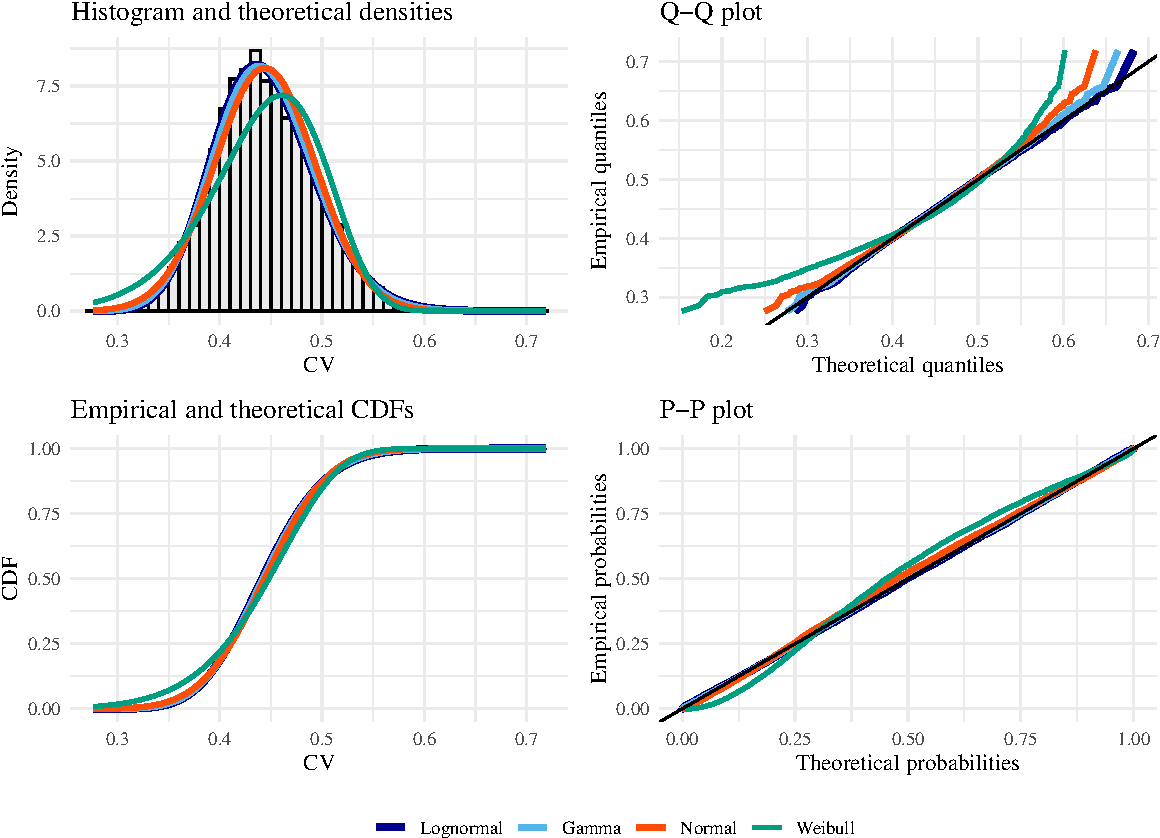
\includegraphics[width=0.8\linewidth]{../../Figures/PDF/Plot_cv_gamma-1} 

}

\caption{Goodness of fit plots for evaluating the best distribution with CV data from $\Gamma_{\text{SAR}}$ (under the null hypothesis), with $n=49$, $L=5$, and $\mu=1$.}\label{fig:Plot_cv_gamma}
\end{figure}

\begin{figure}[H]

{\centering 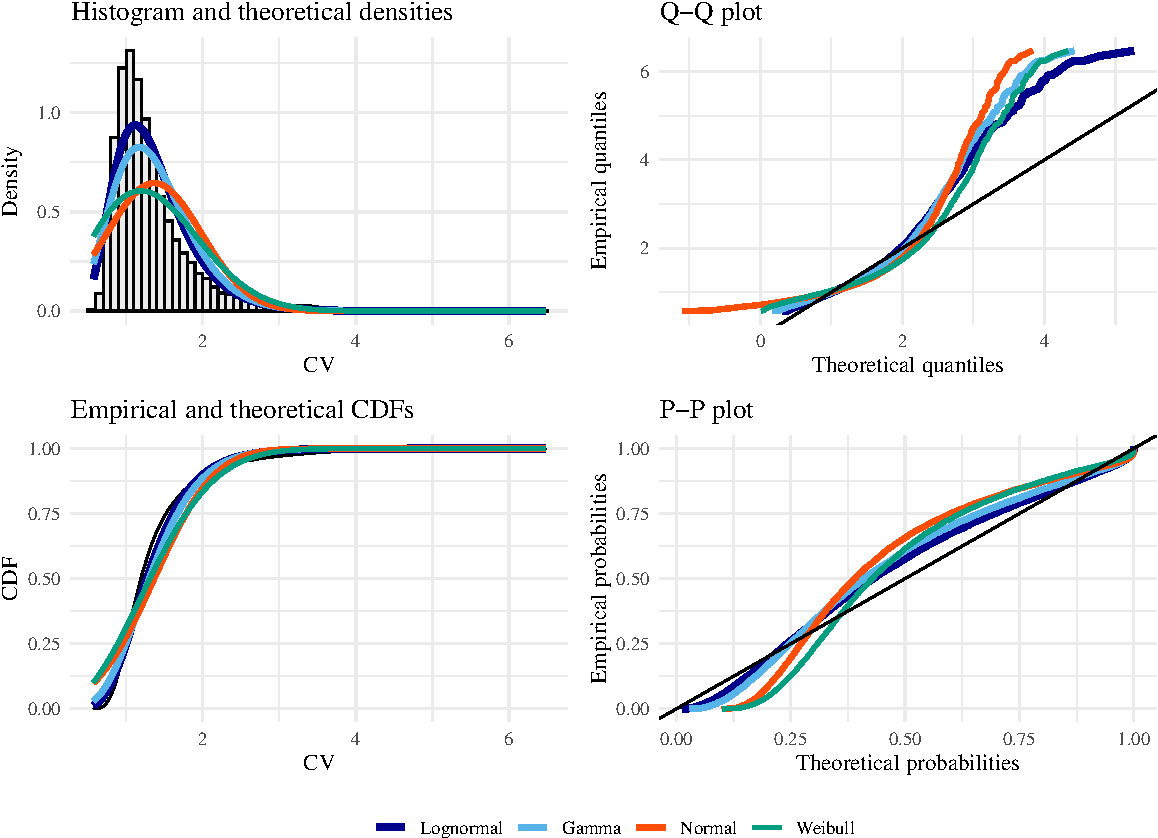
\includegraphics[width=0.8\linewidth]{../../Figures/PDF/Plot_cv-1} 

}

\caption{Goodness of fit plots for evaluating the best distribution with $\text{CV}$ data from $G_I^0$ (under the alternative hypothesis), with  $n=49$, $L=5$, $\mu=1$, and $\alpha=-3$.}\label{fig:Plot_cv}
\end{figure}

\begin{figure}[H]

{\centering 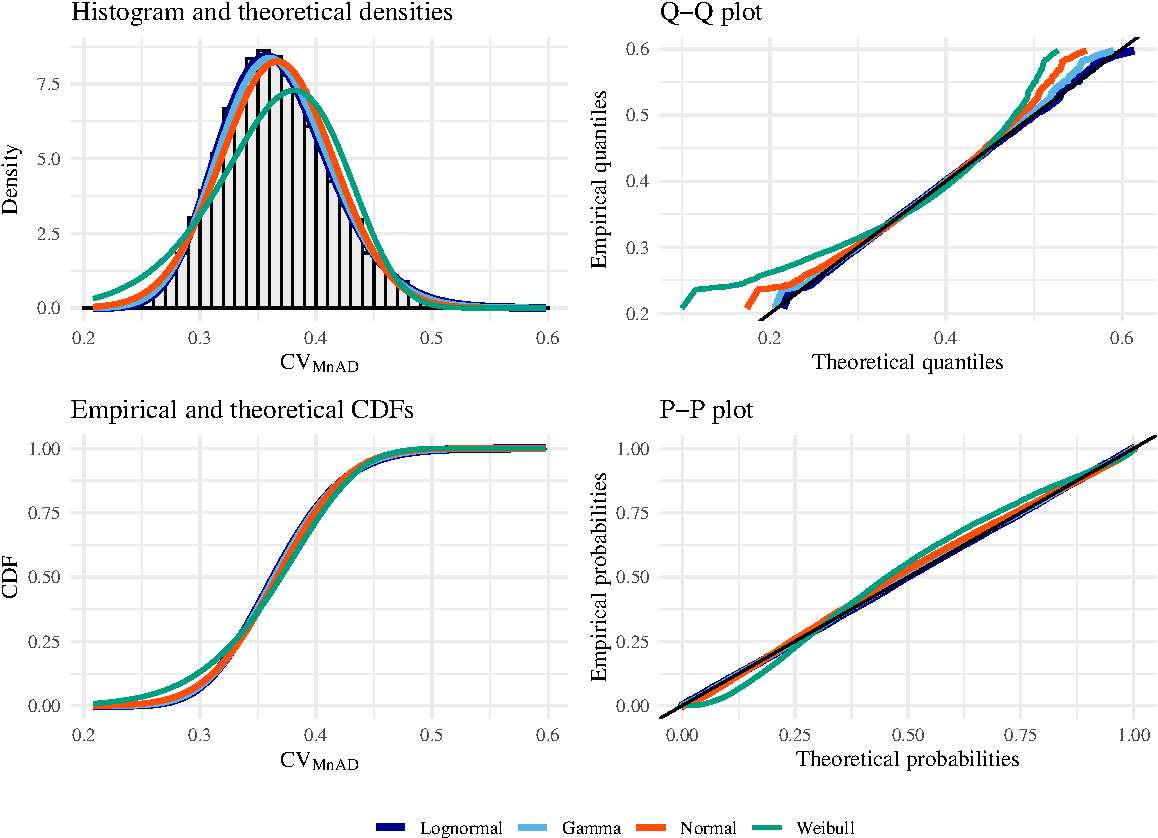
\includegraphics[width=0.8\linewidth]{../../Figures/PDF/Plot_MnADmedian_gamma-1} 

}

\caption{Goodness of fit plots for evaluating the best distribution with $\text{CV}_{\text{MnAD}}$ data from $\Gamma_{\text{SAR}}$ (under the null hypothesis), with  $n=49$, $L=5$, and $\mu=1$.}\label{fig:Plot_MnADmedian_gamma}
\end{figure}
\begin{figure}[H]

{\centering 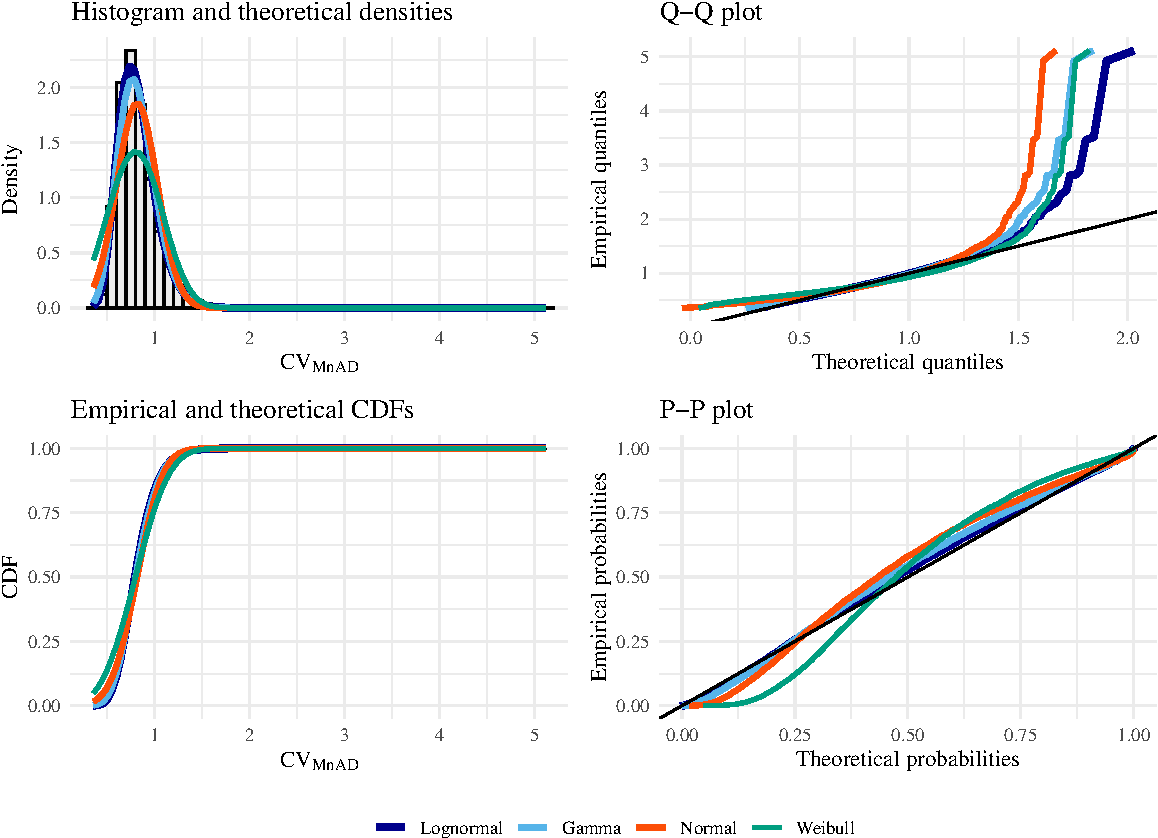
\includegraphics[width=0.8\linewidth]{../../Figures/PDF/Plot_madmed_gi0_MnADmedian-1} 

}

\caption{Goodness of fit plots for evaluating the best distribution with $CV_{\text{MnAD}}$ data from $G_I^0$ (under the alternative hypothesis), with  $n=49$, $L=5$, $\mu=1$, and $\alpha=-3$.}\label{fig:Plot_madmed_gi0_MnADmedian}
\end{figure}

%\begin{figure}[hbt]
%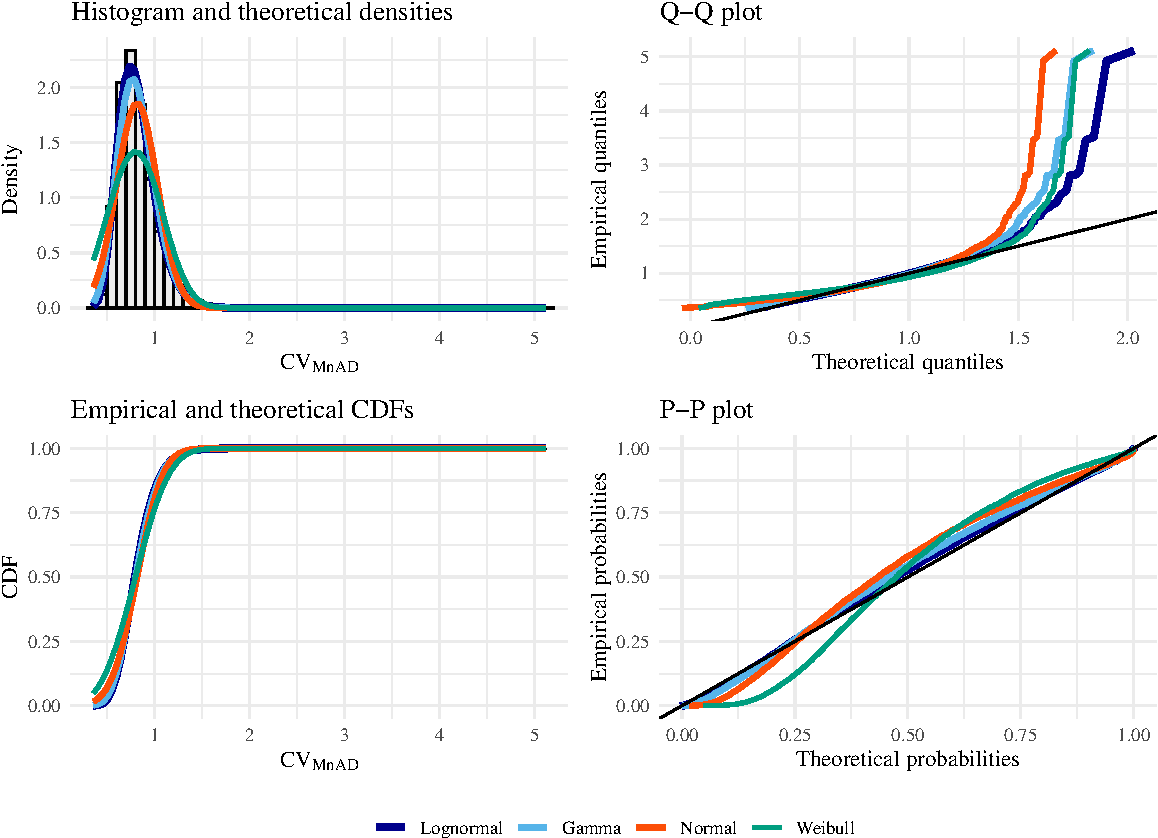
\includegraphics[width=0.8\linewidth]{../../Figures/PDF/Plot_madmed_gi0_MnADmedian-1} \caption{Goodness of fit plots for evaluating the best distribution with $CV_{\text{MnAD}}$ data from $G_I^0$ (under the alternative hypothesis), with  $n=49$, $L=5$, $\mu=1$, and $\alpha=-3$.}\label{fig:Plot_madmed_gi0_MnADmedian}
%\end{figure}